%%% code: 代码文件夹
%%% figures: 图片文件夹
%%% *.cls: LaTeX 格式文件
%%% *.tex: LaTeX 文档文件
%%% *.bib: Bib 引用文献源文件
\documentclass{mcmthesis}  % 文档类型
\mcmsetup{CTeX = false,   % 使用 CTeX 套装时，设置为 true
	tcn = 2602805,   % 队伍控制号
	problem = A,  % 选题
	sheet = true,   % sheet页
	titleinsheet = true,   % sheet页显示标题
	keywordsinsheet = true,  % sheet页显示关键词
	titlepage = false,   % 标题页
	abstract = true  % 摘要
}
%%%%%%%%%%%%%%%%%%%%%%%%%%%%%%%%%%%%%%%%%%%%%%%%%%%%%%%

%%%%%%%%%%%%%%%%%%%%%%%%%%%%%%%%%%%%%%%%%%%%%%%%%%%%%%%
%%% 导入宏包和引用文献源
%%%%%%%%%%%%%%%%%%%%%%%%%%%%%%%%%%%%%%%%%%%%%%%%%%%%%%%
\usepackage{pgfplots}
\pgfplotsset{compat=1.18}
%\usepackage{palatino}  % 帕拉提诺体字体宏包
\usepackage{times}  % 正文使用Times New Roman风格字体
\usepackage{newtxmath}
\usepackage{lipsum}  % 导入生成段落的宏包
\usepackage{indentfirst}
\usepackage{booktabs} % For professional-looking tables
\usepackage{xcolor}   % For cell coloring
\usepackage{colortbl} % Required for \rowcolor
\definecolor{LightGreen}{rgb}{0.9, 0.95, 0.9}
\definecolor{LightPink}{RGB}{255, 229, 237}
\definecolor{LightBlue}{RGB}{229, 238, 255}
\usepackage{fancyhdr}
\usepackage{enumitem} % 用于自定义列表格式
\usepackage{setspace}
\usepackage{svg}
\usepackage{booktabs}  % 三线表加粗
\usepackage{float}
\usepackage{eso-pic}  % 用于在页面添加背景
\usepackage{graphicx} % 图片支持
\usepackage{tikz}     % 用于绘制半透明覆盖层
\usepackage{subcaption}
\usepackage{caption}
\setlist[itemize]{listparindent=2em}
\setlist[enumerate]{listparindent=2em}
\usepackage[titles]{tocloft}
\usepackage{tabularx}
\setlength{\cftbeforesecskip}{6pt}   % 节之前的间距
\setlength{\cftbeforesubsecskip}{3pt} % 小节之前的间距
\newcommand{\upcite}[1]{\textsuperscript{\textsuperscript{\cite{#1}}}}
\urlstyle{rm}
\setlength{\headheight}{13.6pt}

%下面是彩色框设置
\usepackage[most]{tcolorbox}
\tcbuselibrary{breakable}

\usepackage{titlesec}
%\newtcolorbox{titleoff}{%
%	colback=#FDF8EF,
%	colframe=#FCF1E0,
%	fonttitle=\bfseries,
%	title={},
%	breakable,
%	boxrule=0.8pt,
%	left=8pt,
%	right=8pt,
%	top=8pt,
%	bottom=8pt,
%}
	
\newtcolorbox[auto counter,number within=chapter]{titleon}[1][]{%
	colback=cyan!5!white,
	colframe=cyan!75!black,
	fonttitle=\bfseries,
	title=#1,
	breakable,
}
	

%%%%%%%%%%%%%%%%%%%%%%%%%%%%%%%%%%%%%%%%%%%%%%%%%%%%%%%

%%%%%%%%%%%%%%%%%%%%%%%%%%%%%%%%%%%%%%%%%%%%%%%%%%%%%%%
%%% 文档信息设置
%%%%%%%%%%%%%%%%%%%%%%%%%%%%%%%%%%%%%%%%%%%%%%%%%%%%%%%
\title{Beyond the Black Box: A Multifactor Differential Model for Smartphone Power Drain}  % 文章标题
\author{\small Team 2602805}  % 作者，开启标题页才会显示
\date{\today}  % 日期，开启标题页才会显示

%%%%%%%%%%%%%%%%%%%%%%%%%%%%%%%%%%%%%%%%%%%%%%%%%%%%%%%
%%% 文档开始
%%%%%%%%%%%%%%%%%%%%%%%%%%%%%%%%%%%%%%%%%%%%%%%%%%%%%%%
\begin{document}  % 文档
	\begin{abstract}  % 摘要
		
		\vspace*{-12pt}
		In modern life, smartphone battery life is jointly influenced by multiple factors such as user usage intensity, processor load, and ambient temperature, while also constrained by the charging history and aging process of lithium-ion batteries. In response, this paper constructs a continuous-time differential equation model to characterize the temporal dynamic behavior of battery charge, enabling accurate prediction of remaining battery life across diverse usage scenarios.
		
		To begin with, we develop a foundational dynamic differential equation model for SOC. We consider the composition of total power from multiple dimensions, \textbf{clarifying the characteristics of each power component individually}, and further incorporate the influence of temperature to refine and improve the basic model. The \textbf{Runge-Kutta method} is employed to numerically solve the differential equation. Through stochastic simulation, it is found that battery usage duration under a Wi‑Fi network environment is \textbf{10.66  hours}, which aligns with actual smartphone usage patterns, verifying the validity of the proposed model. Finally, we describe the parameter estimation method, further confirming the model's reliability.
		
		Next, we select several typical usage scenarios to perform Time-to-Empty predictions. The results indicate that \textbf{GPS, CPU load, and screen brightness have a significant impact on battery life}, \textbf{with GPS reducing battery life by up to 40.354\%}. We conduct Monte Carlo simulations to analyze the uncertainty of these influencing factors; the \textbf{CV values across different scenarios range between 2\% and 4.5\%}, indicating that the model exhibits strong robustness. Lastly, we evaluate the model's performance through sensitivity analysis.
		
		Then, we validate the reasonableness of the model assumptions and analyze the model's sensitivity. By altering the assumption regarding screen type, we verify \textbf{the model's broad adaptability to different screen types}. Stochastic simulation results based on the thermal-efficiency feedback mechanism reveal that the sensitivity ranking of key usage parameters remains unchanged, and the \textbf{model output varies by only 0.25\%}, confirming the validity of the model assumptions. Sensitivity analysis using SRC, VIF, and CV values yields a \textbf{CV of only 5.52\%}, indicating that the model possesses good stability and reliability. Finally, we analyze \textbf{fluctuations in usage patterns}, and find that \textbf{when the behavior update interval is set to 60 minutes, battery life reaches a maximum of 12.36  hours, representing a 17.4\% improvement over the worst‑case scenario}.
		
		Finally, considering the impact of battery aging, we provide recommendations for users and operating systems. \textbf{We advise users to activate core modules as needed, and recommend that operating systems implement fine‑grained control of core parameters, among other measures}. The model is further applied to a smart band, indicating its \textbf{ability for device generalization}.
		\begin{keywords}  % 关键词
			Differential Equations, Random Simulation, Monte Carlo Simulation, State of Charge (SOC), Battery Life
		\end{keywords}  % 结束关键词
	\end{abstract}  % 结束摘要
	\maketitle  % 生成sheet页
	
	\setcounter{page}{2} % 重置页码为 2
	\tableofcontents  % 生成目录表

	
	%%%%%%%%%%%%%%%%%% sheet页与目录页结束 %%%%%%%%%%%%%%%%%%
	
	\newpage  % 开始新的一页
	\section{Introduction}  % 一级标题
	\subsection{Background}  % 二级标题
	Smartphones are indispensable in modern society, yet their battery performance is highly unpredictable—lasting a full day in some cases and depleting rapidly in others. While heavy usage is often blamed, actual battery drain stems from a complex interplay of factors: screen size and brightness, processor load, network activity, and background apps that consume power even when the device is idle. Environmental factors such as ambient temperature further increase the complexity of the problem: the effective capacity of some batteries decreases in low‑temperature environments, or they may overheat under sustained high loads. Additionally, battery performance is also influenced by usage history and charging habits.
	
	Accordingly, developing an accurate mathematical model for smartphone battery behavior is critical to predicting battery life and optimizing usage strategies. We constructs a continuous-time dynamic model for the state of charge (SOC) of lithium-ion batteries, aiming to characterize the SOC-time functional relationship under real-world usage scenarios and predict remaining usable time across conditions. The model integrates the coupled mechanisms of multi-factor power consumption and accounts for long-term effects like battery aging, thereby providing practical battery management recommendations for users and theoretical support for operating system-level energy-saving strategy design.
	
	\begin{figure}[h!]
		\centering
		% trim = 左边裁剪 下边裁剪 右边裁剪 上边裁剪（单位：cm）
		% clip 表示启用裁剪功能
		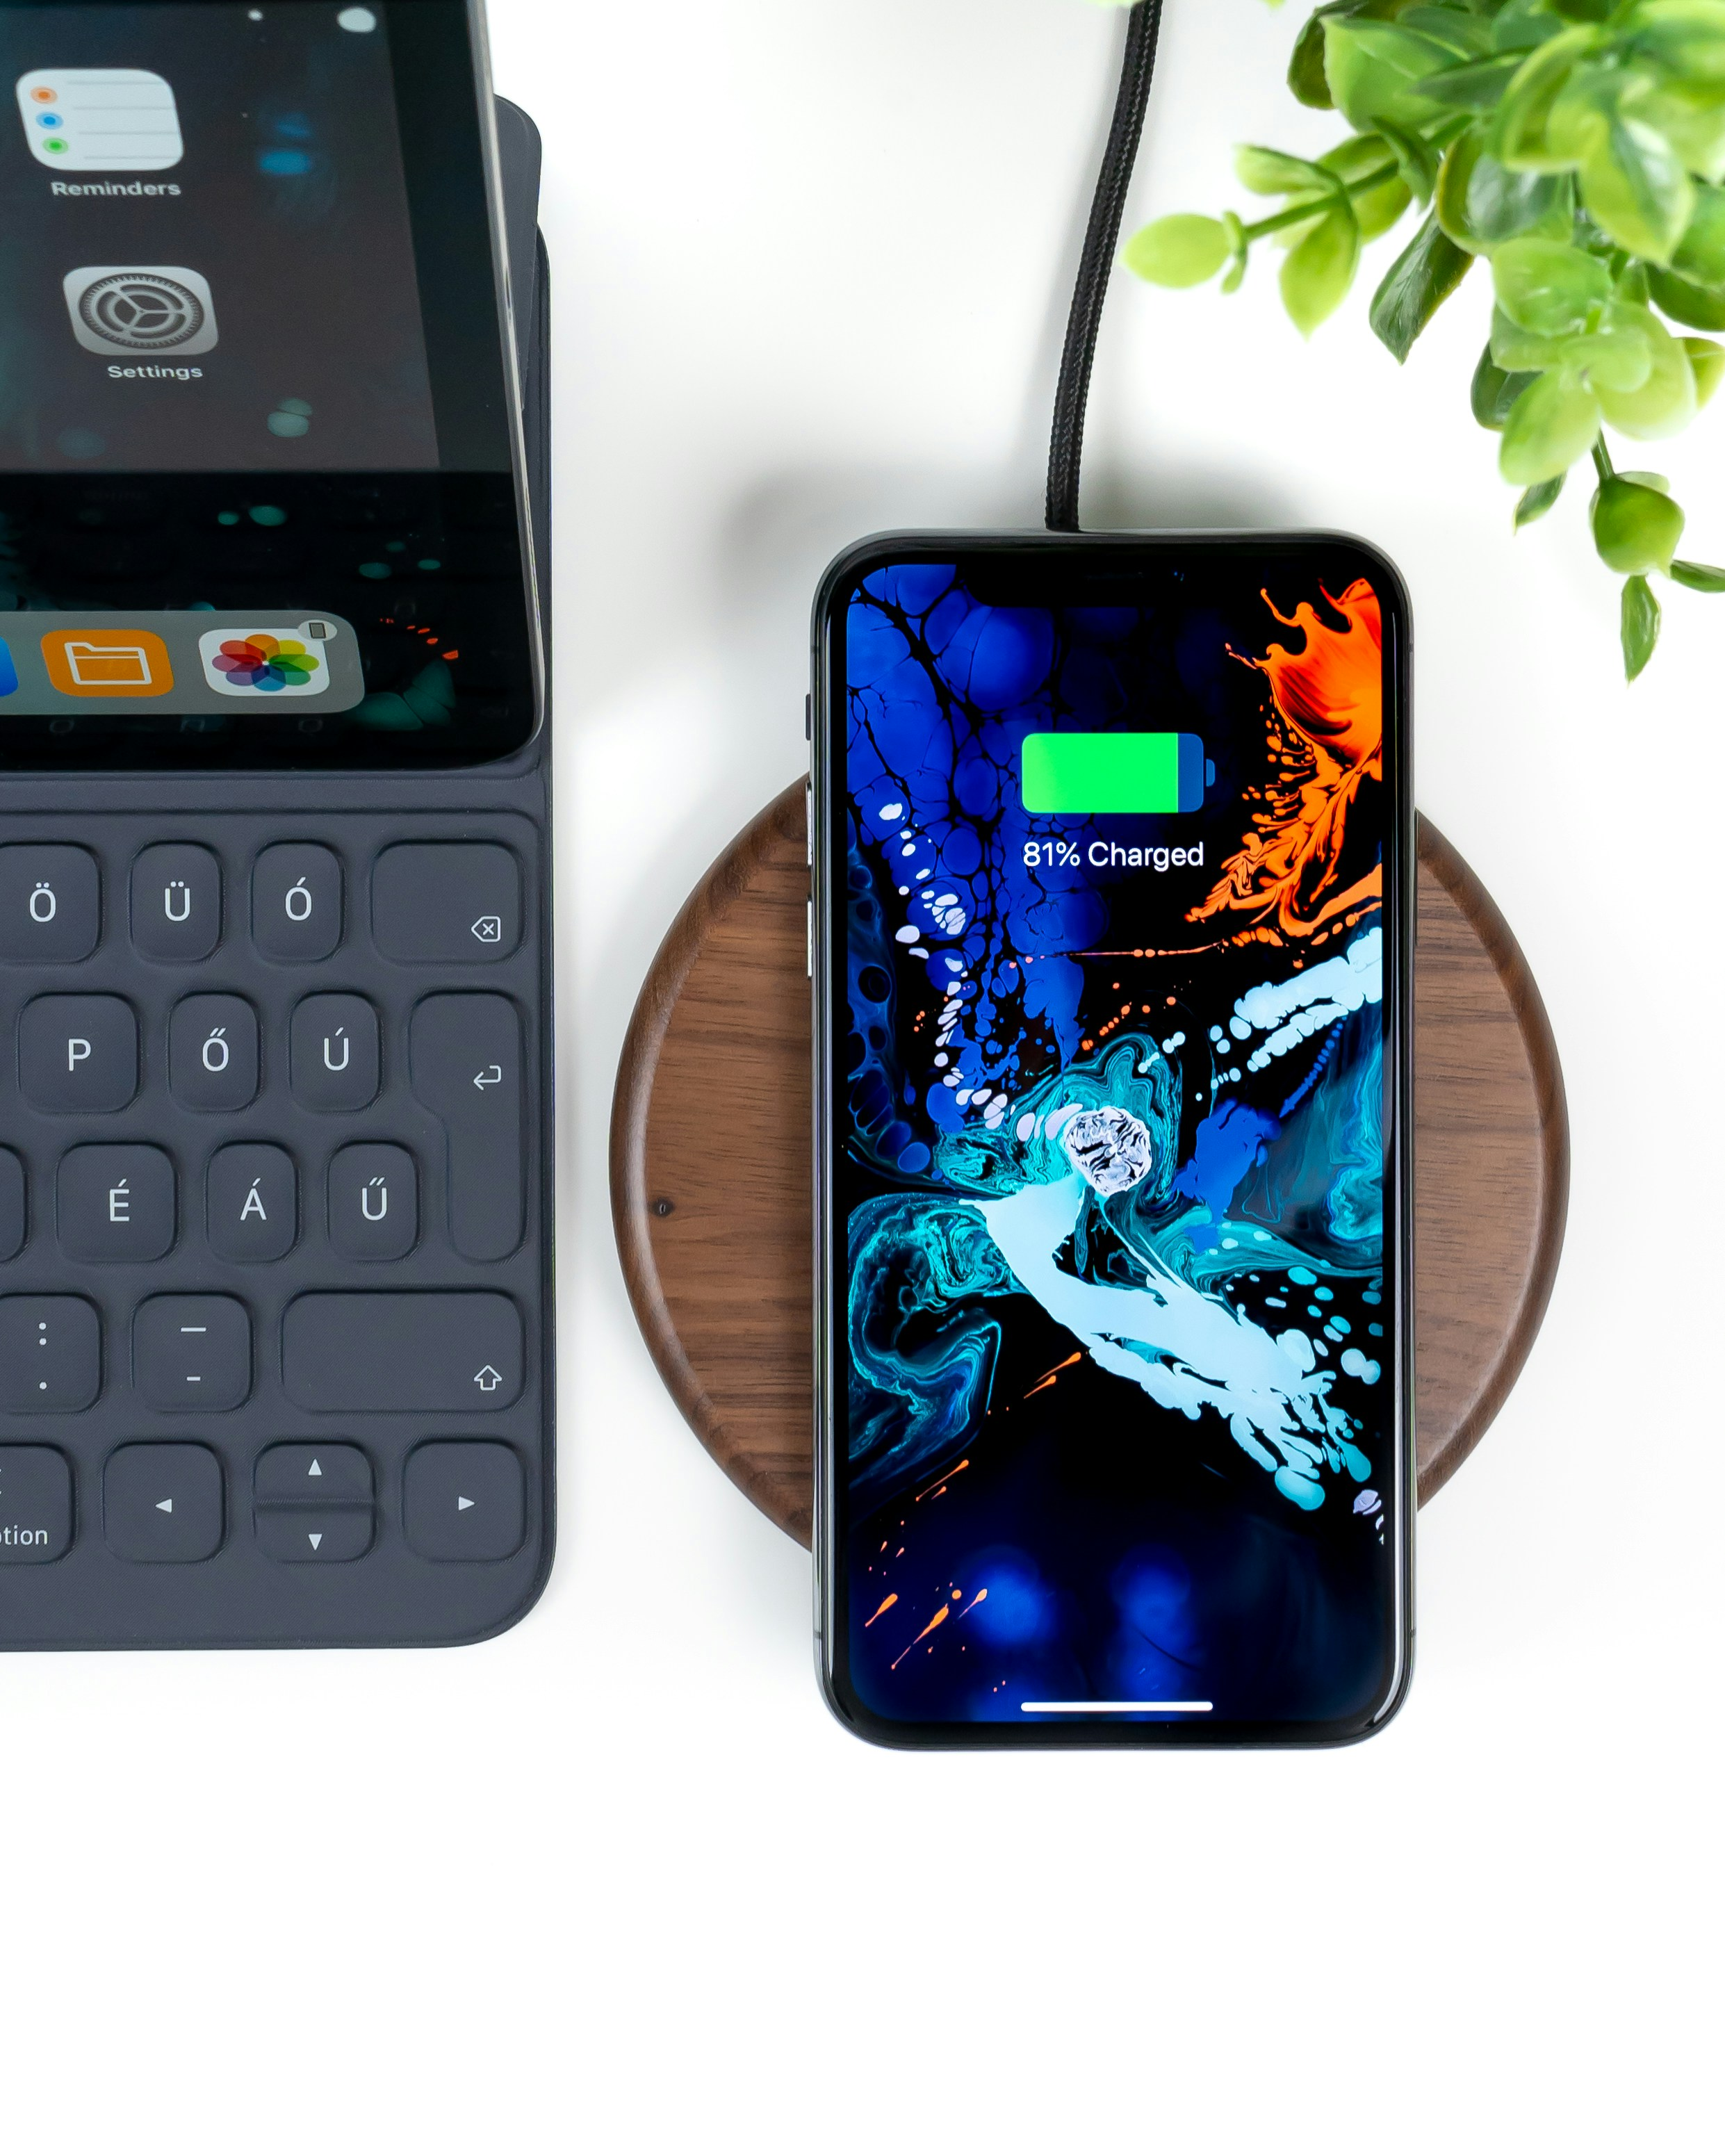
\includegraphics[
		width=0.5\textwidth,
		trim=0cm 15cm 0cm 0cm,  % 仅上方裁剪1厘米，其他边不裁剪
		clip
		]{figures/无线充电.jpg}
		\caption{Charging smartphone battery}
	\end{figure}
	
	\subsection{Restatement of the Problem}
	Based on the basic information and relevant conditions regarding battery discharge described in the problem statement, the following issues need to be addressed:
	\begin{itemize}
		\item Build a continuous-time model of battery power consumption that comprehensively considers various factors, such as screen brightness and background processes. Discrete curve fitting, statistical regression, and other such mathematical forms shall not be adopted.
		\item Use this model to predict the remaining available time under different initial charge levels and usage states, analyze the causes of uncertain outcomes, and systematically evaluate the impact of various usage activities and environmental conditions on battery life and discharge rates.
		\item Conduct a sensitivity analysis of the model. Investigate changes in the model's prediction results after adjusting assumptions, parameter values, and fluctuations in usage patterns, and analyze the model’s strengths and weaknesses.
		\item Provide recommendations for smartphone users on slowing down battery aging, reducing power consumption, extending the device's usage time, etc. Additionally, explain how the model can be applied to other portable devices, such as smart watches.
	\end{itemize}
	
	\subsection{Our Work \& Model Overview}
	\indent After analyzing the problem, our team searched for data and built Battery Power Drain Dynamic Model to solve it. To avoid a complicated description and clearly show our work process, the flow chart is presented in Figure \ref{fig:2026美赛流程图}.
	
	Considering the background, we analyze and solve the problems step-by-step:
	
	\textbf{Step 1}: \textbf{Establish a basic dynamic differential equation model for battery state of charge.}
	
	\textbf{Step 2}: \textbf{Extend the model to incorporate multiple influencing factors.} Include factors such as CPU load, background processes, network status, screen brightness, and ambient temperature, while accounting for power consumption differences between OLED and LCD screen types and GPS operating status. Construct the differential equation and solve it using the RK method.
	
	\textbf{Step 3}: \textbf{Model prediction and result analysis.} Use the model to predict the remaining battery power under different initial charge levels and usage scenarios. Compare the predictions with actual observed data, analyze the sources of prediction discrepancies, and systematically evaluate the impact of various usage activities and environmental conditions on battery discharge rate and battery life.
	
	\textbf{Step 4}: \textbf{Sensitivity analysis and model stability testing.} Investigate the sensitivity of prediction results by adjusting model assumptions, introducing SRC, VIF, and CV to explore key parameters, and varying the frequency of switching patterns to examine the fluctuation of usage patterns. Assess the robustness and reliability of the model under different conditions.
	
	\textbf{Step 5}: \textbf{User recommendations and model generalization.} Based on the modeling results, provide users with actionable battery usage recommendations to reduce energy consumption, extend battery life, and delay battery aging. Further explore the applicability and potential of this model for other portable devices such as  smartwatches.
	
	For better arranging our process of problem solving, the flow diagram of our work is shown in Figure \ref{fig:2026美赛流程图}.
	
	\begin{figure}[h!]
		\centering
		% trim = 左边裁剪 下边裁剪 右边裁剪 上边裁剪（单位：cm）
		% clip 表示启用裁剪功能
		\vspace{-0.6cm}
		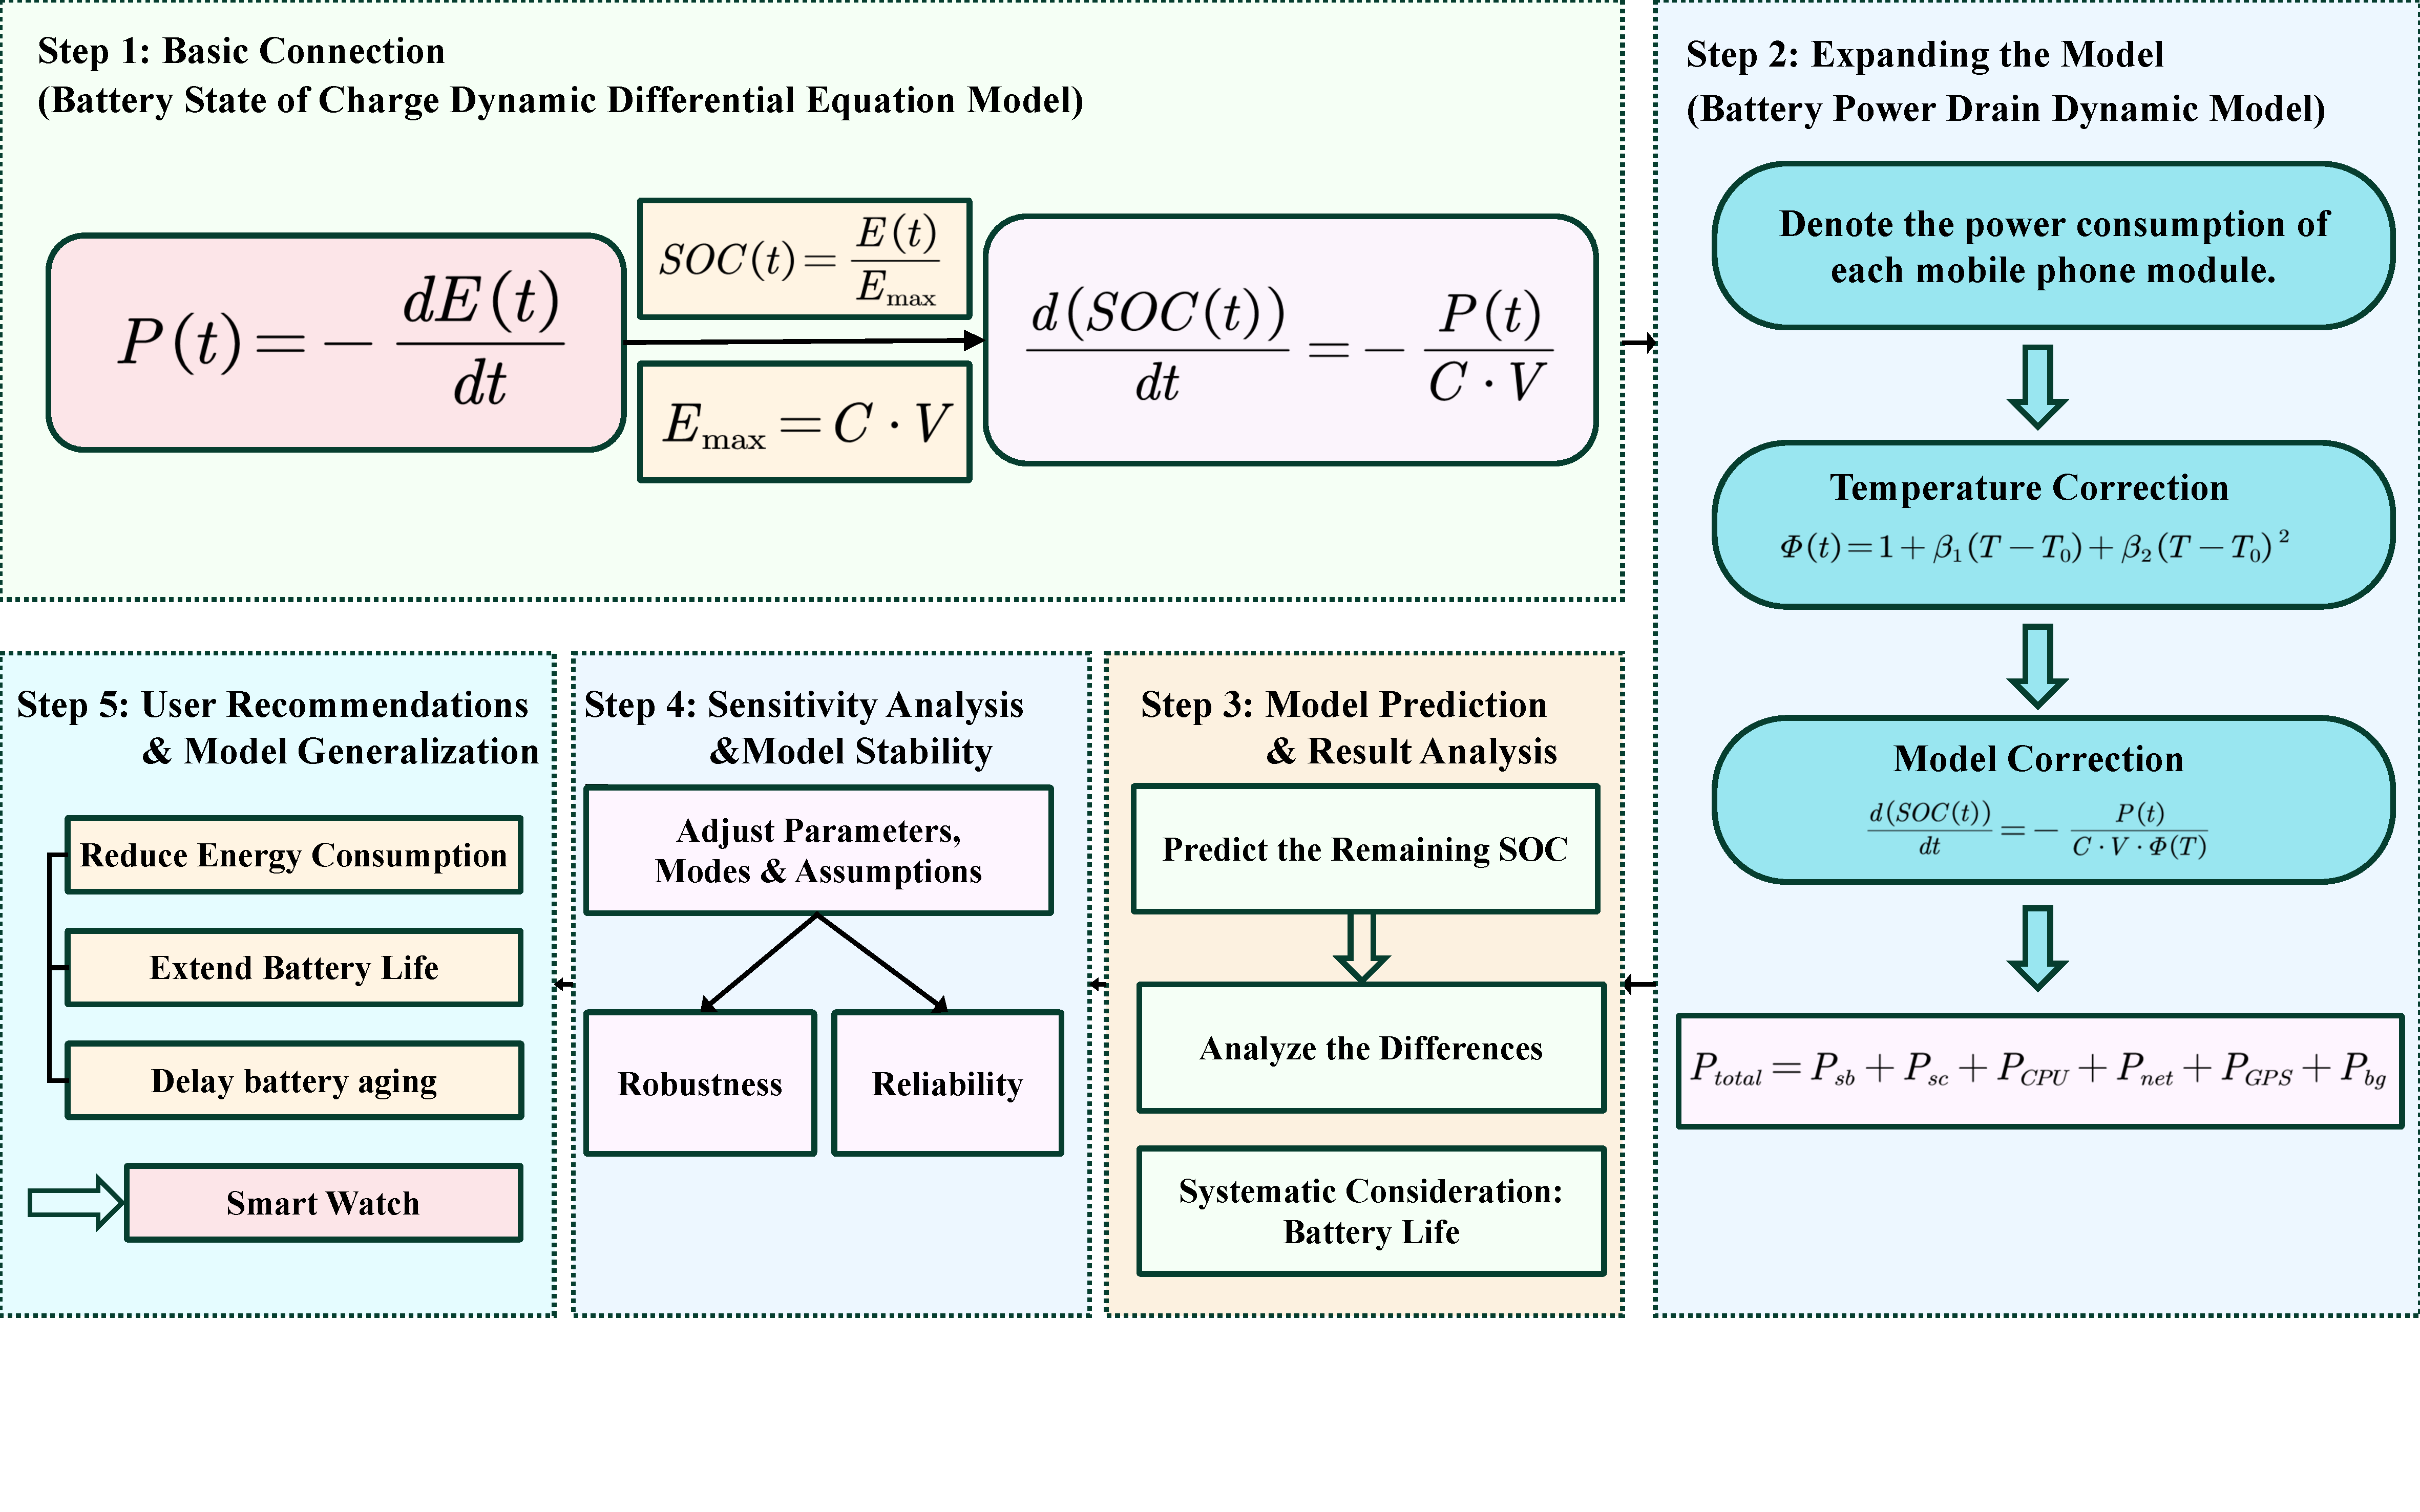
\includegraphics[
		width=1\textwidth,
		trim=0cm 6.5cm 0cm 0cm, 
		clip
		]{figures/2026美赛流程图.pdf}
		\caption{Flow Chart of Our Work}
		\label{fig:2026美赛流程图}
	\end{figure}
	
	
	\section{Assumptions and Justifications}  % 一级标题
	Given the potential complexity of real-world scenarios, we begin by introducing several reasonable assumptions to make the problem tractable. Each assumption is accompanied by a corresponding justification as follows:
	\begin{itemize}
		\item \textbf{Assumption:} The temperature is assumed to be constant under the same usage scenario when building the model.
		\\
		\textbf{Justification:} Within the time scale of regular usage, smart terminals have effective heat dissipation capabilities, so the device temperature can be regarded as approximately constant under given environmental conditions.
		
		\item \textbf{Assumption:} Remaining charge prediction is performed using an OLED screen.
		\\
		\textbf{Justification:} OLED screens are currently prevalent, making the prediction results more aligned with practical applications.
		
		\item \textbf{Assumption:} Remaining charge is estimated separately for each fixed network environment.
		\\
		\textbf{Justification:} In practical usage scenarios, network connections undergo relatively few changes.
		
		\item \textbf{Assumption:} Coupling effects between modules are not considered.
		\\
		\textbf{Justification:} The synergistic and offsetting effects between modules have a minor impact on power consumption and are already reflected in the power consumption of individual modules.
		
		\item \textbf{Assumption:} The phone is equipped with a lithium-ion battery.
		\\
		\textbf{Justification:} The majority of modern smartphones are powered by lithium-ion batteries.
	\end{itemize}
	
	\newpage
	\section{Notations}  % 一级标题
	
	The key notations used in this paper are listed in Table \ref{tab:notations}.
	\begin{table}[h!]
		\centering
		\vspace{-7pt}
		\caption{Notations used in this paper}
		\label{tab:notations}
		\renewcommand{\arraystretch}{1.2} 
		\begin{tabular}{lcl}
			\toprule
			\textbf{Symbol} & \textbf{Definition} & \textbf{Unit} \\
			\midrule
			\rowcolor{LightGreen}
			$SOC(t)$ & State of Charge at time $t$ & $\%$ \\
			$P(t)$ & Total power consumption at time $t$ & W \\
			\rowcolor{LightGreen}
			$C$ & Rated battery capacity & mAh \\
			$V$ & Nominal battery voltage & V \\
			\rowcolor{LightGreen}
			$P_{\text{standby}}$ & Standby power & W \\
			$B(t)$ & Normalized screen brightness & $-$ \\
			\rowcolor{LightGreen}
			$\alpha_{\text{OLED}}, \gamma_{\text{OLED}}$ & OLED screen power coefficients & $-$ \\
			$\alpha_{\text{LCD}}$ & LCD screen power coefficient & $-$ \\
			\rowcolor{LightGreen}
			$k(t)$ & Black pixel proportion on OLED & $-$ \\
			$\eta$ & OLED dark content reduction coefficient & $-$ \\
			\rowcolor{LightGreen}
			$u(t)$ & CPU utilization rate & $\%$ \\
			$\beta_{\text{freq}}, \beta_{\text{idle}}$ & CPU power coefficients & $-$ \\
			\rowcolor{LightGreen}
			$\tau(t)$ & Network load intensity at time $t$ & $-$ \\
			$P_{\text{net}}^{\text{Wi-Fi}}, P_{\text{net}}^{4\text{G}}, P_{\text{net}}^{5\text{G}}$ & Network power functions & W \\
			\rowcolor{LightGreen}
			$P_{\text{GPS}}(t)$ & GPS power consumption & W \\
			$P_{\text{bg}}(t)$ & Background app power & W \\
			\rowcolor{LightGreen}
			$N_g, N_s, N_v$ & Background app counts & $-$ \\
			$\omega_g, \omega_s, \omega_v$ & App type weights & $-$ \\
			\rowcolor{LightGreen}
			$\Phi(T)$ & Temperature correction coefficient & $-$ \\
			$T, T_0$ & Battery and reference temperatures & $^\circ$C \\
			\bottomrule
		\end{tabular}
	\end{table}
	
	\vspace*{-15pt}
	\section{Battery Power Drain Dynamic Model} 
	
	To make the model more consistent with practical scenarios, we retrieved relevant data online to revise the model coefficients. The data sources are shown in Table \ref{数据来源}.
	
	\begin{table}[h!]
		\centering
		\caption{Data Sources}
		\label{数据来源}
		\renewcommand{\arraystretch}{1}
		\renewcommand{\heavyrulewidth}{1.2pt}
		\begin{tabular}{p{6.5cm}p{8cm}}
			\toprule
			\textbf{Data Type} & \textbf{URL Link} \\
			\midrule
			\rowcolor{LightBlue}
			Screen Luminous Characteristic Data & {\small\url{https://displaymate.com/Smartphone_ShootOut_1.htm?utm_source#Highlights}} \\
			Background power consumption difference coefficient among different application categories & {\footnotesize\url{https://www.phonearena.com/news/these-apps-silently-drain-your-smartphone-battery_id177012}} \\
			\bottomrule
		\end{tabular}
		\renewcommand{\heavyrulewidth}{0.8pt}
	\end{table}
	
	\vspace*{-5pt}
	\subsection{Model Selection}
	\begin{itemize} [listparindent=2em]
		\item \textbf{Rejection of the Electrochemical Model:}
		
		In the field of battery modeling, equivalent circuit models and electrochemical models are commonly used to characterize the terminal voltage dynamics, polarization effects, and battery aging processes. However, the modeling objective of this task is not to accurately depict the internal physical processes of the battery, but to analyze the impacts of different functional modules on power consumption and their effects on the evolution of State of Charge (SOC) from the perspective of user behavior.
		
		In practical usage scenarios, the information accessible to users is mainly the functional usage status and power consumption, rather than state variables such as battery terminal voltage, current, or internal temperature. Therefore, introducing a battery mechanism model that relies on current and voltage is not only difficult for parameter calibration but also significantly increases model complexity and reduces model interpretability.
		
		\item \textbf{Adoption of the Model for Battery Power Consumption:}
		
		To align with real-world applications and enable convenient parameter calibration with practical data, this study adopts a first-order SOC evolution model based on the law of energy conservation. The focus is placed on the structured modeling of power terms. By characterizing the behavior-driven power consumption characteristics of modules including the screen, CPU, and network, an effective description of the relationship between user behavior and power consumption is achieved.
		\end{itemize}
	
	\subsection{A comprehensive multi-factor power consumption function}
	First, based on the basic relationships $SOC(t)=\frac{E(t)}{E_{\max}}$ and $E_{\max}=C\cdot V$, we establish a preliminary differential equation for battery power consumption:
	\begin{equation}
		\frac{d(SOC(t))}{dt} = -\frac{P(t)}{C \cdot V}
	\end{equation}
	
	\begin{titleoff}
		\begin{equation}
			\frac{d(SOC(t))}{dt} = -\frac{P(t)}{C \cdot V}
		\end{equation}
	\end{titleoff}
	
	\begin{titleon}[Theorem]
		\begin{equation}
			\frac{d(SOC(t))}{dt} = -\frac{P(t)}{C \cdot V}
		\end{equation}
	\end{titleon}
	
	We decompose the total power into standby power, screen usage power, CPU operating power, network operating power, GPS power consumption and background application power consumption:
	\begin{equation}
		P_{total}=P_{standby}+P_{screen}+P_{CPU}+P_{network}+P_{GPS}+P_{background}
	\end{equation}
	
	Next, we clarify the composition of each power component one by one:
	\begin{enumerate}[label=\bfseries\arabic*.]
		\item \textbf{Standby Power $P_{standby}$}
		
		Standby power refers to the basic power consumption for a mobile phone to maintain system operation when the screen is off and there is no active user operation, independent of the presence of background applications. Research findings indicate that the baseline power consumption of an idle mobile phone is approximately 268 mW; for the sake of subsequent analysis, a value of 0.27 W can be adopted\upcite{1}, which is defined as follows:
		\begin{equation}
			P_{standby}=0.27W
		\end{equation}
		
		\item \textbf{Screen Usage Power $P_{\text{screen}}$}
		
		Screen power consumption is positively correlated with brightness and screen-on duration. We establish power consumption models for OLED and LCD screens respectively:
		\begin{enumerate}[label=(\arabic*)]
			\vspace*{-7pt}
			\item 
			OLED is a self-luminous device. The power consumption fluctuates significantly with the brightness and color proportion of displayed content and is positively correlated with brightness\upcite{2}. Since the luminous power of OLED pixels has a nonlinear correlation with brightness\upcite{3}, a quadratic term $B(t)^2$ is introduced for fitting. Considering the power-saving effect of dark content, the power consumption model is established as follows:
			
			\vspace*{-7pt}
			\begin{equation}
				P_{\text{screen,OLED}}(t) = \left( \alpha_{\text{OLED}} B(t) + \gamma_{\text{OLED}} B(t)^2 \right) \left( 1 - \eta k(t) \right)
			\end{equation}
			where $P_{\text{screen,OLED}}(t)$ is the instantaneous operating power of the OLED screen at time $t$; $\alpha_{\text{OLED}}=0.7\mathrm$ and $\gamma_{\text{OLED}}=0.3\mathrm$ are the linear and nonlinear power consumption coefficients of brightness, respectively; $\eta=0.8$ is the power consumption attenuation coefficient of dark content; $k(t)$ is the proportion of black pixels at time $t$ with the value range of $[0,1]$; $B(t)$ is the normalized brightness value at time $t$. The model is simplified as:
			\vspace*{-7pt}
			\begin{equation}
				P_{\text{screen,OLED}}(t) =\left( 0.7B(t) + 0.3B(t)^2 \right) \left( 1 - 0.8k(t) \right)
			\end{equation}
			
			\vspace*{-7pt}
			\item 
			LCD relies on an LED backlight layer for light supply. Pixels only adjust light transmittance while the backlight layer remains on continuously, with power consumption dominated by backlight brightness. Basic backlight power consumption still exists in full-black display. Screen power consumption has a significant linear correlation with brightness\upcite{4} and a weak correlation with screen area. The power consumption model is established as follows:
			\vspace{-5pt}
			\begin{equation}
				P_{\text{screen,LCD}}(t) = \alpha_{\text{LCD}} B(t)
			\end{equation}
			where $P_{\text{screen,LCD}}(t)$ is the instantaneous operating power of the LCD screen at time $t$; $\alpha_{\text{LCD}}=0.9\mathrm{W}$ is the brightness power consumption coefficient; $B(t)$ is the normalized brightness value at time $t$. The model is simplified as:
			\vspace{-5pt}
			\begin{equation}
				P_{\text{screen,LCD}}(t) = 0.9 B(t)
			\end{equation}
			
			\begin{figure}[h!]
				\centering
				\renewcommand{\arraystretch}{1}
				\subcaptionbox{Screen Power Consumption\label{fig:Screen Power Consumption}}%
				{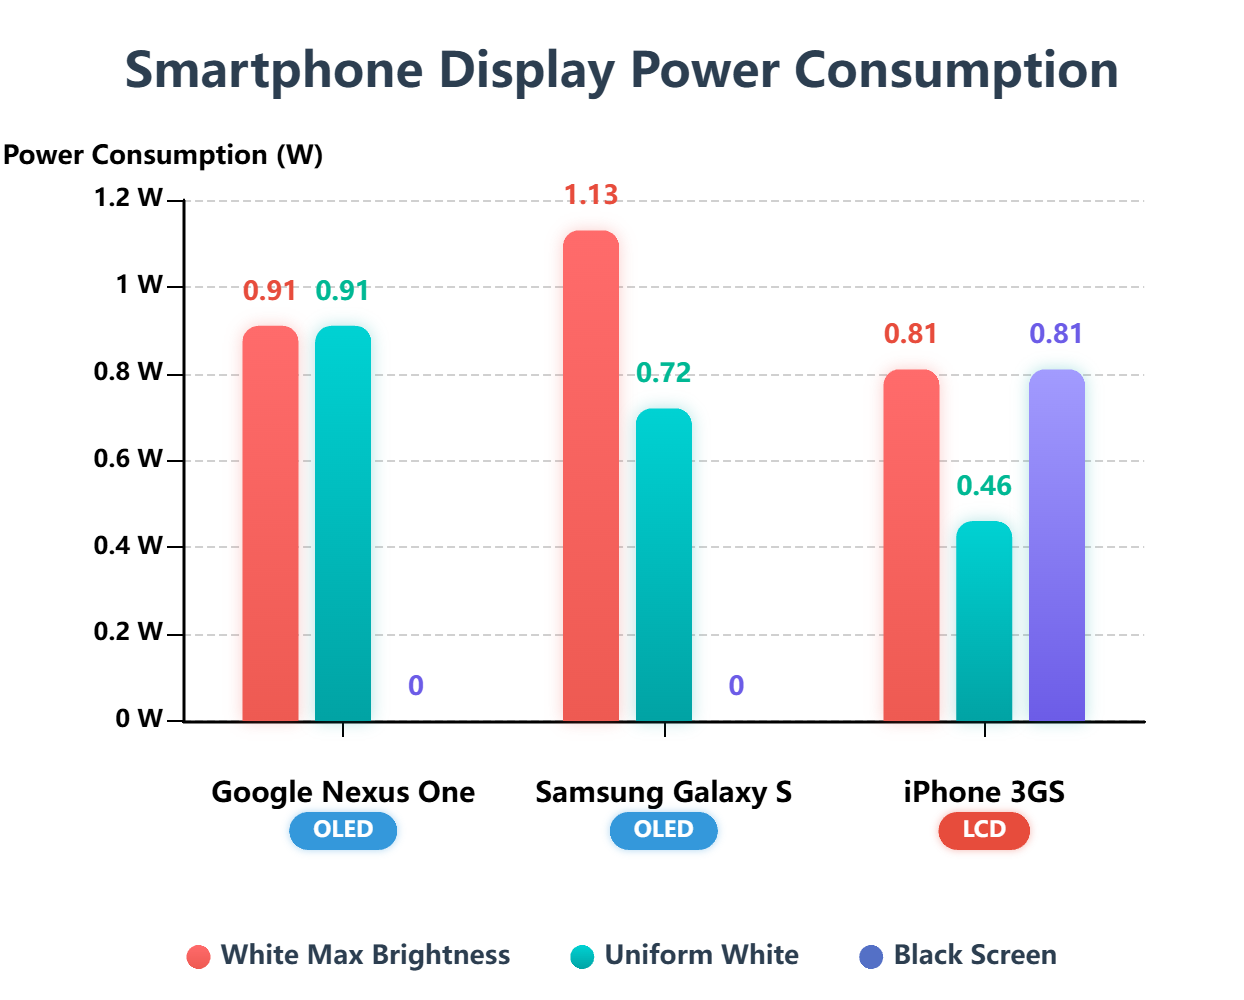
\includegraphics[width=.3\textwidth]{figures/OLED.png}}%
				\hspace{60pt} % 自定义间距，10pt约3.5mm
				\subcaptionbox{The common value of $B(t)$\label{fig:The common value of $B(t)$}}%
				{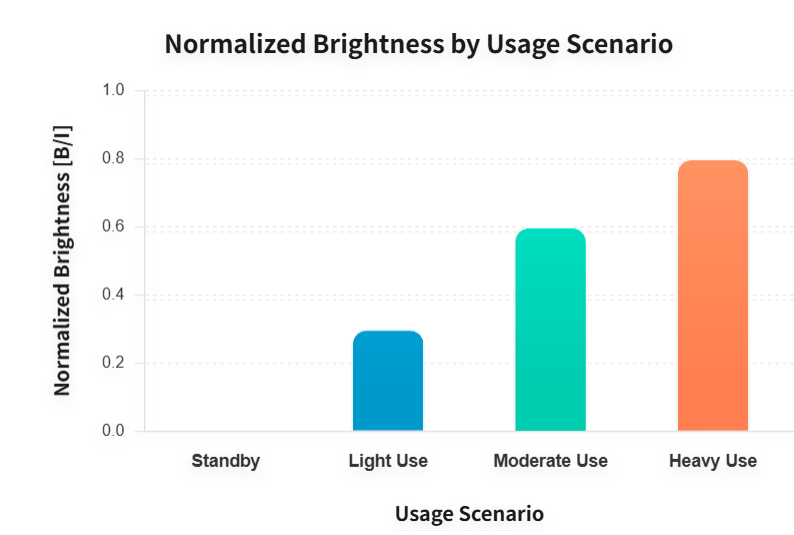
\includegraphics[width=.3\textwidth]{figures/B.png}}
				\renewcommand{\arraystretch}{1.5}
				\caption{Screen-related data}
			\end{figure}
			
		\end{enumerate}
		
		
		\item \textbf{CPU operating power $P_{CPU}$}
		
		The CPU operating power is the power consumption of the processor when executing tasks and performing data operations, which has a strong correlation with the CPU utilization rate (the ratio of the time the CPU executes non-idle processes to the total running time)
		
		A quantitative relationship between CPU utilization rate and power consumption can be established by regulating the CPU utilization rate, and the specific regulation process is shown in Figure \ref{fig:CPU}.
		\begin{figure}[h!]
			\centering
			\vspace{-5pt}
			% trim = 左边裁剪 下边裁剪 右边裁剪 上边裁剪（单位：cm）
			% clip 表示启用裁剪功能
			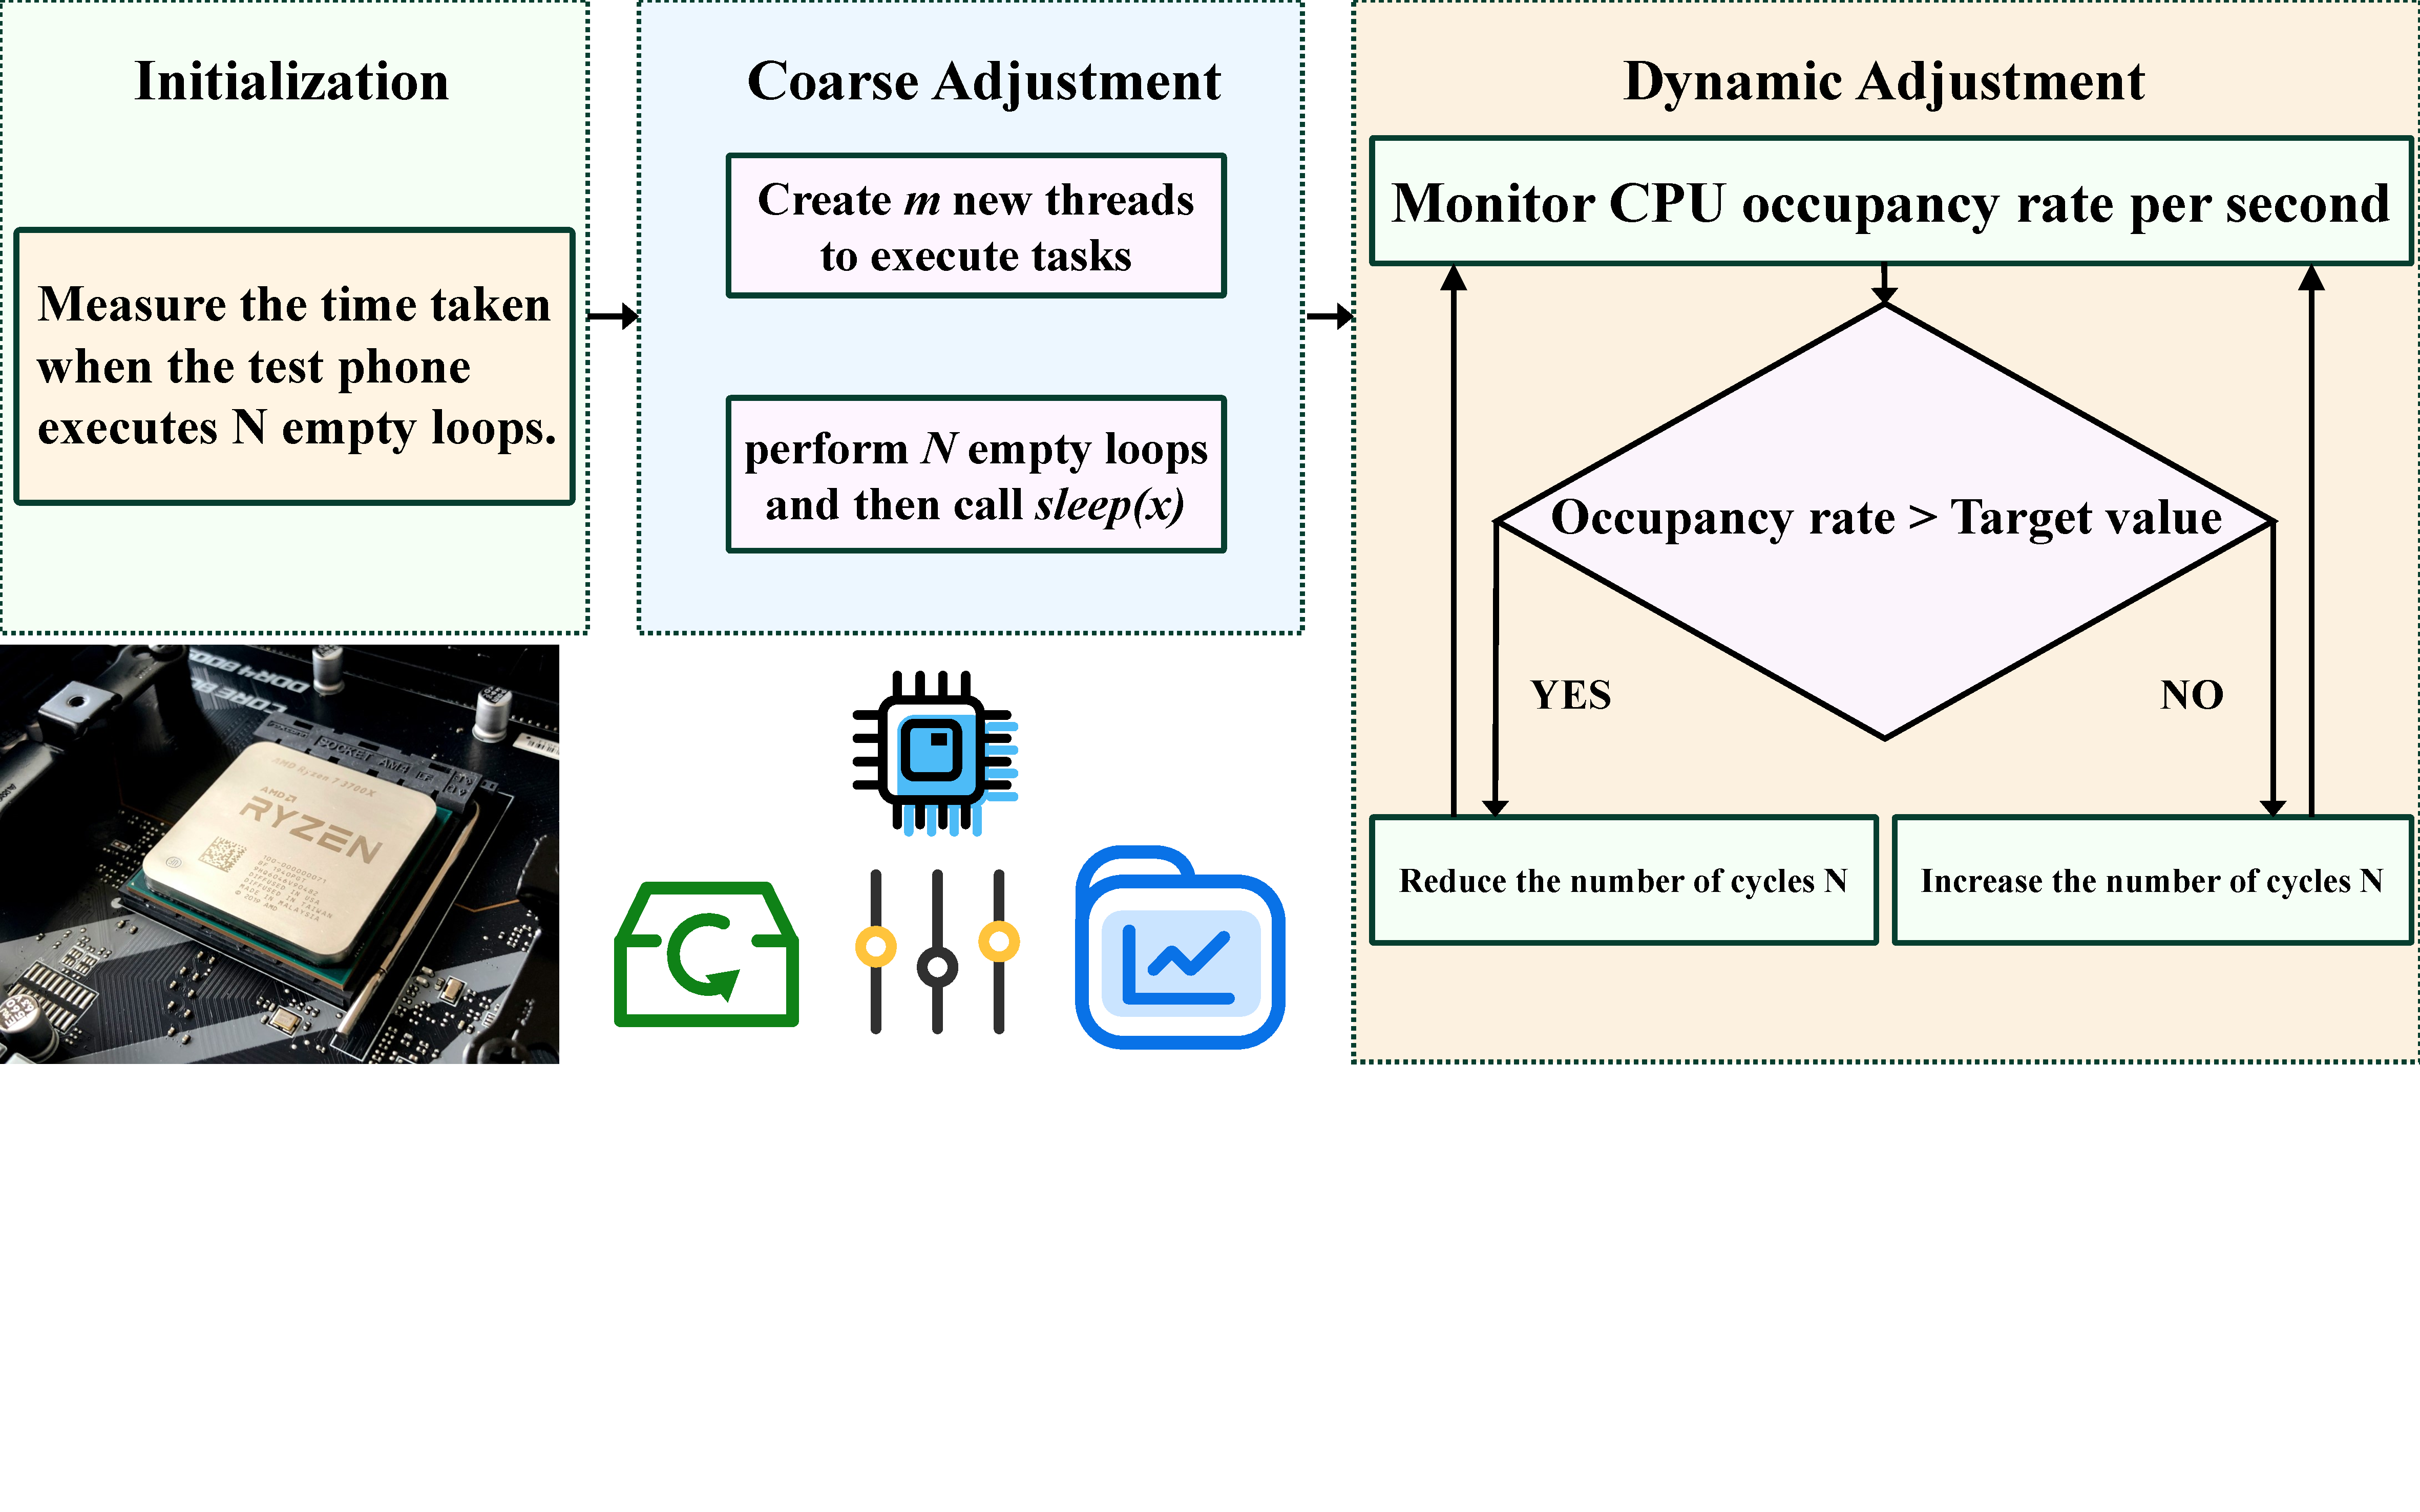
\includegraphics[
			width=0.8\textwidth,
			trim=0cm 14cm 0cm 0cm, 
			clip
			]{figures/CPU.pdf}
			\caption{CPU Occupancy Rate Control Process}
			\label{fig:CPU}
		\end{figure}
		
		In summary, the CPU power consumption model is constructed as follows:
		\begin{equation}
			P_{CPU}(t)=\beta_{freq}u(t)+\beta_{idle}
		\end{equation}
		where $P_{CPU}(t)$ denotes the instantaneous power consumption of the CPU, $u(t)$ is the CPU utilization rate with $u(t)\in[0,1]$, $\beta_{freq}$ is the dynamic power consumption coefficient related to the CPU utilization rate, and $\beta_{idle}$ is the idle power consumption of the CPU. According to the power consumption characteristics of modern mobile phones, we take $\beta_{freq}=0.8\ \text{W}$ and $\beta_{idle}=0.2\ \text{W}$\upcite{5}, then the CPU power consumption model is simplified as:
		\begin{equation}
			P_{CPU}(t)=0.8u(t)+0.2
		\end{equation}
		\item \textbf{Network operating power $P_{network}$}
		
		Network operating power refers to the power consumed by mobile phones during data transmission and signal interaction via mobile networks and Wi-Fi. Based on statistical data analysis \upcite{6}, a linear fitting model is adopted to characterize this power consumption. Considering the distinct power characteristics associated with different network connection types (Wi-Fi, 4G, 5G), we establish mathematical power models for each network type:
		
		\begin{equation}
			P_{\text{network}}(\tau(t)) = a_{\text{network}} \tau(t) + b_{\text{network}}
		\end{equation}
		where $P_{\text{network}}(\tau(t))$ denotes the instantaneous operating power of the network; $\tau(t)$ denotes the network load intensity (ranging from $[0,1]$); $a_{\text{network}}$ is the load-dependent power coefficient, and $b_{\text{network}}$ is the baseline operating power. The parameters are calibrated based on empirical measurements from the literature, yielding $a_{\text{Wi-Fi}}=0.18\,\mathrm{W}$, $b_{\text{Wi-Fi}}=0.08\,\mathrm{W}$, $a_{4\text{G}}=0.507\,\mathrm{W}$, $b_{4\text{G}}=0.15\,\mathrm{W}$, $a_{5\text{G}}=0.65\,\mathrm{W}$, and $b_{5\text{G}}=0.15\,\mathrm{W}$. Consequently, the model can be simplified as:
		
		\begin{equation}
			\begin{cases}
				P_{\text{network}}^{\text{Wi-Fi}}(\tau(t)) = 0.18\tau(t) + 0.08 \\
				P_{\text{network}}^{4\text{G}}(\tau(t)) = 0.507\tau(t) + 0.15 \\
				P_{\text{network}}^{5\text{G}}(\tau(t)) = 0.65\tau(t) + 0.15
			\end{cases}
		\end{equation}
		
		
		\item \textbf{GPS power consumption $P_{GPS}$}
		
		GPS power consumption is the power consumed by a mobile phone when its GPS module is activated for positioning and navigation, and it is one of the core power consumption items in location service scenarios. Its power consumption is directly related to the positioning mode: the GPS module works continuously with high power consumption in high-precision positioning mode (e.g., real-time navigation, trajectory recording); while it operates intermittently with significantly lower power consumption in low-power positioning mode (e.g., background rough positioning, check-in). We considered the impact of GPS on power consumption under different operational modes. Based on the actual power consumption characteristics of the GPS module in modern mobile phones, its mathematical model is established as follows\upcite{5}:
		\begin{equation}
			P_{\text{GPS}}(t) =
			\begin{cases}
				0, & \text{GPS off} \\
				0.0492, & \text{GPS on} \\
				0.4449, & \text{GPS in navigation mode}
			\end{cases}
		\end{equation}
		
		\item \textbf{Background application power consumption} $P_{background}$
		
		Background app power consumption is the hidden power consumption generated by apps running in the background of smartphones. Such apps consume power continuously through background data refreshing, message pushing and other operations, and their power consumption is significantly correlated with the number and type of running background apps, with real-time networked apps having much higher background power consumption. It is also directly affected by factors such as app wake-up frequency and data transmission volume.
		
		To fit practical scenarios, this study classifies mainstream background apps into three typical categories: games, social media and video apps, based on their operational characteristics and differences in background power consumption. Combining the ideas of linear weighting and normalization, a universal mathematical model for background app power consumption is established as follows:
		\begin{equation}
			P_{\text{bg}}(t) = \delta_{bg,0} + \frac{\delta_{bg}}{N_{bg,\text{max}}} \left( \omega_g N_g(t) + \omega_s N_s(t) + \omega_v N_v(t) \right)
		\end{equation}
		where $\delta_{bg,0}$ denotes the basic background power consumption, representing the fixed power consumption term of the system background mechanism; \footnotesize
		$
		\frac{\delta_{bg}}{N_{bg,\text{max}}} \left( \omega_g N_g(t) + \omega_s N_s(t) + \omega_v N_v(t) \right)
		$
		\normalsize is the dynamic power consumption increment introduced by background apps, reflecting the power consumption variation caused by the number and type of apps; $N_g(t), N_s(t), N_v(t)$ are the numbers of game, social, and video apps running in the background at time $t$, respectively, serving as the core input variables of the model; $\omega_g, \omega_s, \omega_v$ are the dimensionless power weight coefficients of game, social, and video apps, respectively, which are used to quantify the differentiated impacts of different app types on background power consumption.
		
		To enhance the practical fitting performance and reliability of the model, this study is based on publicly available measured data from Table \ref{数据来源}. Through data fitting and weight optimization calculations, the power weight coefficients for the three types of applications are determined as: $(\omega_g, \omega_s, \omega_v) = (0.23, 0.32, 0.45)$. Consequently, the final model for background application power consumption is:
		\begin{equation}
			P_{\text{bg}}(t) = \delta_{bg,0} + \frac{\delta_{bg}}{N_{bg,\text{max}}} \left( 0.23 N_g(t) + 0.32 N_s(t) + 0.45 N_v(t) \right)
		\end{equation}
		
		Given that the synergistic and offsetting effects among modules are minor, and to some extent reflected in the variations of individual modules, we do not investigate the interactions between modules.
		
	\end{enumerate}
		
		\subsection{Model Modification Considering Temperature Effects}
		
		Given the nonlinear temperature dependence of smartphone battery performance—with accelerated degradation at extreme temperatures—a temperature correction term is added to the model:
		\begin{equation}
			\frac{d\,\text{SOC}(t)}{dt} = -\frac{P_{\text{total}}(t)}{C \cdot V \cdot \Phi(T)}
		\end{equation}
		\begin{equation}
			\Phi(T) = 1 + \beta_1(T - T_0) + \beta_2(T - T_0)^2
		\end{equation}
		where $T$ is the battery's current operating temperature, $T_0$ is the reference temperature taken as $25^\circ\text{C}$, and $\Phi(T)$ is the temperature correction coefficient, which is a dimensionless quantity representing the ratio of the system's actual performance at the current temperature $T$ to its performance at the reference temperature $T_0$. $\beta_1$ and $\beta_2$ are the linear and quadratic temperature coefficients, respectively, obtained by fitting a quadratic polynomial to the experimental data using the ordinary least squares method. The specific procedure is as follows:
		
		\textbf{Step 1.} Set $T$ as independent variable, $C(T)/C(T_0)$ as dependent variable;
		
		\textbf{Step 2.} Minimize the objective function:
		\begin{equation}
			\min_{\beta_1,\beta_2} \sum_{i=1}^{n} \left[ \frac{C(T_i)}{C(T_0)} - \left(1 + \beta_1(T_i - T_0) + \beta_2(T_i - T_0)^2\right) \right]^2
		\end{equation}
			
		\textbf{Step 3.} Derive normal equations by setting partial derivatives of the objective function (w.r.t. $\beta_1, \beta_2$) to zero, then solve for optimal coefficients.
		
		Through data fitting, $\beta_1=-0.004$ and $\beta_2=-0.00006$ are obtained and used for subsequent quantitative analysis\upcite{7}.
	
	\subsection{Using the Runge-Kutta method to solve the numerical solution of ODEs}
	
	In summary, the system of differential equations describing the variation of the state of charge (SOC) of the mobile phone battery is constructed as follows:
	\begin{equation}
		\left\{
		\begin{aligned}
			&\frac{d\,\text{SOC}(t)}{dt} = -\frac{P_{\text{total}}(t)}{C \cdot V \cdot \Phi(T)}
			\\
			&P_{\text{total}}(t) = P_{\text{standby}} + P_{\text{screen}}(t) + P_{\text{CPU}}(t) + P_{\text{network}}(t) + P_{\text{GPS}}(t) + P_{\text{background}}(t) \\
			&P_{\text{standby}}=0.27W
			\\
			&P_{\text{screen,OLED}}(t) = \left( \alpha_{\text{OLED}} B(t) + \gamma_{\text{OLED}} B(t)^2 \right) \left( 1 - \eta k(t) \right)
			\\
			&P_{\text{screen,LCD}}(t) = \alpha_{\text{LCD}} B(t) 
			\\
			&P_{CPU}(t)=\beta_{freq}u(t)+\beta_{idle} 
			\\
			&P_{\text{network}}(\tau(t)) = a_{network}\tau(t) + b_{network}
			\\
			&P_{\text{GPS}}(t) =
			\begin{cases}
				0W, & \text{GPS off} \\
				0.0492W, & \text{GPS on} \\
				0.4449W, & \text{GPS in navigation mode}
			\end{cases}
			\\
			&P_{\text{bg}}(t) = \delta_{bg,0} + \frac{\delta_{bg}}{N_{bg,\text{max}}} \left( \omega_g N_g(t) + \omega_s N_s(t) + \omega_v N_v(t) \right)
			\\
			&\Phi(T) = 1 + \beta_1(T - T_0) + \beta_2(T - T_0)^2
		\end{aligned}
		\right.
	\end{equation}
	
	Substituting the relevant parameters, the parameterized system of differential equations is obtained as follows:
	\begin{equation}
		\left\{
		\begin{aligned}
			&\frac{d\,\text{SOC}(t)}{dt} = -\frac{P_{\text{total}}(t)}{C \cdot V \cdot \Phi(T)} 
			\\
			&P_{\text{total}}(t) = P_{\text{standby}} + P_{\text{screen}}(t) + P_{\text{CPU}}(t) + P_{\text{network}}(t) + P_{\text{GPS}}(t) + P_{\text{background}}(t) 
			\\
			&P_{\text{standby}}= 0.27W\\
			&P_{\text{screen,OLED}}(t) =\left( 0.7B(t) + 0.3B(t)^2 \right) \left( 1 - 0.8k(t) \right) 
			\\
			&P_{\text{screen,LCD}}(t) = 0.9 B(t)
			\\
			&P_{CPU}(t)=0.8u(t)+0.2 
			\\
			&P_{\text{network}}^{\text{Wi-Fi}}(\tau(t)) = 0.18\tau(t) + 0.08
			\\
			&P_{\text{network}}^{4\text{G}}(\tau) = 0.507\tau(t) + 0.15  
			\\
			&P_{\text{network}}^{5\text{G}}(\tau(t)) = 0.65\tau(t) + 0.15
			\\
			&P_{\text{GPS}}(t) =
			\begin{cases}
				0W, & \text{GPS off} \\
				0.0492W, & \text{GPS on} \\
				0.4449W, & \text{GPS in navigation mode}
			\end{cases}
			\\
			&P_{\text{bg}}(t) = \delta_{bg,0} + \frac{\delta_{bg}}{N_{bg,\text{max}}} \left( 0.23 N_g(t) + 0.32 N_s(t) + 0.45 N_v(t) \right)
			\\
			& \Phi(T) = 1 + 0.004(T - T_0) + 0.00006(T - T_0)^2,\quad \Phi(T) > 0
		\end{aligned}
		\right.
	\end{equation}
	
	\begin{equation}
		T_{\text{battery life}} = \int_{0}^{\text{SOC}_0} \frac{C \cdot V \cdot \phi(T)}{P_{\text{total}}(t)} \, d(\text{SOC})
	\end{equation}
	
	We use the fourth-order Runge--Kutta (RK) method to solve the differential equation. As a single-step method suitable for equations lacking analytical solutions, it achieves high accuracy through a weighted average of slopes at discrete points, without requiring high-order derivatives. Numerical solutions are obtained by evaluating the right-hand side of the equation multiple times\upcite{8}. Its \textbf{fourth-order accuracy} satisfies engineering requirements for battery modeling. The RK method handles nonlinear functions composed of multiple modules using only evaluations of \( P(t) \), offering \textbf{low computational cost}, \textbf{no need for historical data}, and \textbf{strong stability}, effectively avoiding the numerical instability of explicit Euler under long-term integration and random disturbances.
	
	\subsection{Stochastic Simulation}
	To fit practical scenarios, we conducts stochastic simulation tests on the established model based on parameters of mainstream mobile phones in the US market (battery capacity 4000 mAh, nominal voltage 3.8 V). The optimal battery operating temperature is selected, with network modes fixed as WiFi, 4G and 5G. First, other factors affecting power consumption are set to change synchronously and randomly every 20 minutes. The simulation results are shown in Figure \ref{fig:同步变化的随机仿真}, and the relevant performance metrics are presented in Table \ref{tab:controlled_comparison}.
	
	\begin{table}[h!]
		\centering
		\caption{Statistical data from random simulation of synchronized parameter changes}
		\label{tab:controlled_comparison}
		\renewcommand{\arraystretch}{1}
		\begin{tabularx}{0.9\textwidth}{lXXX} 
			\toprule
			\textbf{Metric} & \textbf{Wi-Fi} & \textbf{4G} & \textbf{5G} \\
			\midrule
			\rowcolor{LightGreen}
			Total discharge time (h) & 10.66 & 9.51 & 9.18 \\
			Avg SOC decay rate (h$^{-1}$) & 0.0938 & 0.1051 & 0.1089 \\
			\rowcolor{LightGreen}
			Time to 50\% SOC (h) & 5.66 & 5.15 & 5.02 \\
			\bottomrule
		\end{tabularx}
	\end{table}
	
	\begin{figure}[h!]
		\centering
		\vspace*{0pt}
		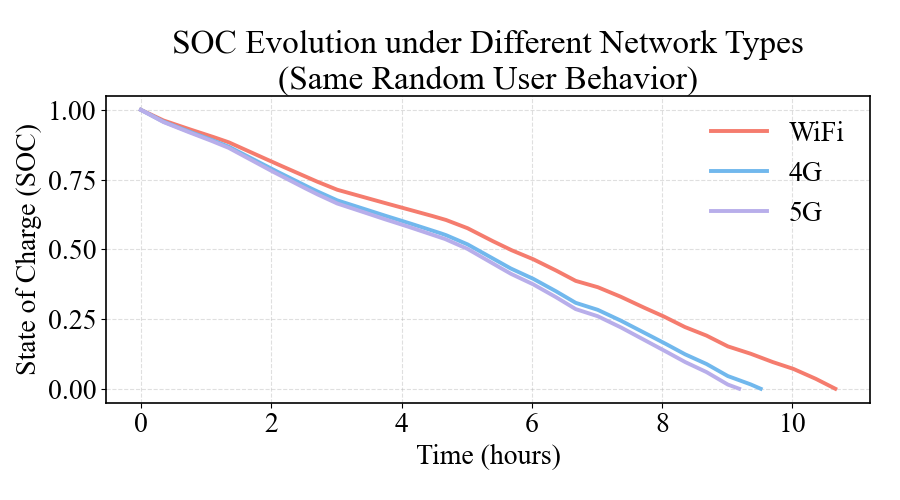
\includegraphics[width=0.4\textwidth,trim=0cm 0.4cm 0cm 0cm,clip]{figures/同步变化的随机仿真.png}
		\caption{Stochastic Simulation with Synchronous Variation}
		\label{fig:同步变化的随机仿真}
	\end{figure}
	
	
	\vspace*{-10pt}
	As shown in Figure \ref{fig:同步变化的随机仿真}, the battery SOC decreases continuously over time under all network modes, with the fastest decay in 5G, followed by 4G and the slowest in WiFi. This rule remains stable throughout the discharge process without curve crossing, which is highly consistent with practical scenarios. Since other energy consumption items are consistent, the result difference can be clearly attributed to the power consumption of different network standards: WiFi achieves low power consumption through short distance and low transmission power, while cellular networks require continuous signaling interaction with base stations, and the high throughput characteristic of 5G further increases energy consumption.
	
	On this basis, a second simulation is carried out with the temperature and network modes unchanged, and other power consumption factors set to change asynchronously and independently every 20 minutes. The results are shown in Figure \ref{fig:独立变化的随机仿真} and Table \ref{tab:realistic_comparison}.
	
	\begin{table}[h!]
		\centering
		\caption{Statistical data from random simulation of independent parameter changes}
		\label{tab:realistic_comparison}
		\renewcommand{\arraystretch}{1} 
		\begin{tabularx}{0.9\textwidth}{lXXX} 
			\toprule
			\textbf{Metric} & \textbf{Wi-Fi} & \textbf{4G} & \textbf{5G} \\
			\midrule
			\rowcolor{LightGreen}
			Total discharge time (h) & 10.92 & 9.72 & 9.23 \\
			Avg SOC decay rate (h$^{-1}$) & 0.0915 & 0.1028 & 0.1083 \\
			\rowcolor{LightGreen}
			Time to 50\% SOC (h) & 5.40 & 4.95 & 4.70 \\
			\bottomrule
		\end{tabularx}
	\end{table}
	
	\begin{figure}[h!]
		\centering
		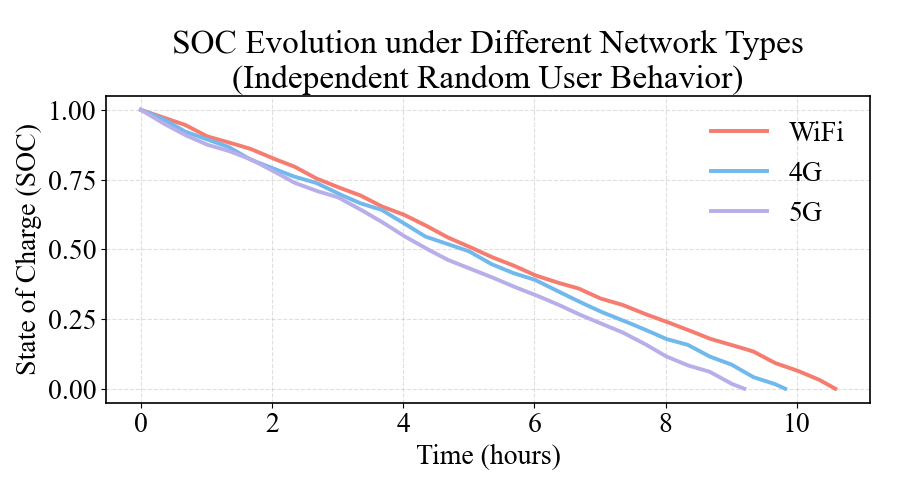
\includegraphics[width=0.5\textwidth,trim=0cm 0.4cm 0cm 0cm,clip]{figures/独立变化的随机仿真.png}
		\caption{Stochastic Simulation with Independent Variation}
		\label{fig:独立变化的随机仿真}
	\end{figure}
	
	Compared with the synchronous simulation, the SOC curve shows more significant random fluctuations, and the 4G decay rate briefly exceeds 5G in some periods. However, on the whole, 5G still discharges to 0\% SOC first, followed by 4G and WiFi, indicating that the influence of network standards on energy consumption is dominant in long-term statistics. The model maintains a stable energy consumption order after introducing multi-source random disturbances, reflecting good robustness.
	
	\subsection{Parameter Estimation Method and Model Rationality Analysis}
	
	\begin{enumerate}[label=\bfseries\arabic*.]
		\item \textbf{Overview of Common Methods}: In system modeling and parameter calibration, common estimation methods include maximum likelihood estimation (MLE), ordinary least squares (OLS), Bayesian estimation, gradient descent, genetic algorithms and other optimization methods.
		
		\textbf{Reasons for Not Adopting}:
		
		\begin{enumerate}[label=\textbf{(\arabic*)}]
			\item \textbf{Scarcity of Data and Structural Complexity:} Smartphone power consumption is a complex large system with multi-factor coupling, making it difficult to collect synchronous power consumption data of each module in practical scenarios. The model is a multivariable nonlinear differential equation; traditional fitting methods (e.g., OLS) require a large amount of time-series data and are prone to unstable results due to noise interference. Bayesian estimation and similar methods need reliable data to support prior or posterior distributions, which is not applicable here.
			\item \textbf{Priority of Model Physical Meaning over Pure Data-Driven Approach:} The model emphasizes interpretability and physical consistency (e.g., the nonlinear relationship between screen power consumption and brightness, and the linear relationship between CPU power consumption and utilization rate are supported by literature on hardware characteristics). Machine learning methods  are "black-box" models that cannot explain the physical meaning of parameters and are prone to overfitting with small samples.
			\item \textbf{Dominant Role of Literature Data as Prior Knowledge:} The power consumption coefficients of each module (e.g., $\alpha_{\text{OLED}}=0.7\text{W}$, $\beta_{\text{freq}}=0.8\text{W}$) have been supported by numerous experimental studies. Directly adopting literature values ensures the basic rationality of the model and avoids large deviations caused by estimation from scratch.
		\end{enumerate}
		
		\item \textbf{Parameter Calibration Method Based on Normalized Behavioral Variables}
		
		Given the lack of large-scale measured data, we adopts a parameter calibration method based on normalized behavioral variables. This approach first normalizes behavior variables that cannot be directly measured (such as screen brightness, CPU utilization, and network load) to the range of $[0,1]$ to eliminate dimensional effects. Subsequently, power consumption models are constructed in a modular manner, with coefficients derived from the mean values or fitting results of empirically measured data in the literature, ensuring that each component of the model has clear physical significance. Finally, to avoid the limitations of machine learning methods-such as high demand for labeled data, poor generalization ability, and lack of physical interpretability of parameters—this method is built on a mechanism-driven foundation, balancing interpretability and engineering applicability.
		
		\item \textbf{Measured Data Correction and Parameter Determination Standards}
		
		The key data sources in the model are clearly defined and adhere to the following standards:
		\begin{enumerate}[label=\textbf{(\arabic*)}]
			\item \textbf{Data Screening and Verification:} Prefer literature data published in recent years with clear experimental conditions and sufficient sample sizes; perform cross-validation on data from different sources to eliminate obvious outliers.
			\item \textbf{Parameter Fitting and Determination:} Directly adopt typical values reported in the literature for modules with significant linear relationships (e.g., LCD screens, CPU idle power consumption); use quadratic term fitting for nonlinear parts (e.g., the brightness-power consumption relationship of OLED screens), where coefficients $\alpha_{\text{OLED}}=0.7$ and $\gamma_{\text{OLED}}=0.3$ are obtained by fitting literature data with the OLS method; the temperature correction coefficient $\beta=-0.004$ is derived from the statistical results of lithium battery temperature effect experiments.
			\item \textbf{Model Correction and Verification:} Use stochastic simulations to verify whether the model output is consistent with practical experience (e.g., 5G power consumption $>$ 4G $>$ Wi-Fi); use control variable simulations to verify whether the ranking of power consumption contributions of each module conforms to common sense.
		\end{enumerate}
	\end{enumerate}
	
	
	\section{SOC Prediction and Uncertainty Quantification}  
	
	\subsection{SOC Prediction}
	
	\vspace*{-5pt}
	Most real-life scenarios are considered. In the subsequent analysis, the network connection is fixed to WiFi, and 5 smartphone usage scenarios are simulated, with the parameters for each scenario shown in Table \ref{tab:指标}:
	
	\begin{table}[h!]
		\centering
		\renewcommand{\arraystretch}{1}
		\caption{Correspondence Table of Device Usage Modes and Parameters}
		\label{tab:指标}
		\begin{tabularx}{0.9\textwidth}{lXXXXX} 
			\toprule
			Usage Mode & $B(t)$ & $u(t)$ & $\tau$ & $P_{GPS}$ & $P_{background}$ \\
			\midrule
			\rowcolor{LightBlue}
			Standby     & 0   & 0    & 0 & 0.049 & 0.08 \\
			Light Usage & 0.3 & 0.25 & 0.2 & 0.049 & 0.09 \\
			\rowcolor{LightBlue}
			Moderate Usage & 0.6 & 0.55 & 0.6 & 0.049 & 0.09 \\
			Heavy Usage & 0.8 & 0.9  & 1 & 0.049 & 0.11 \\
			\rowcolor{LightBlue}
			Navigation Mode & 0.6 & 0.55 & 0.6 & 0.45  & 0.09 \\
			\bottomrule
		\end{tabularx}
	\end{table}
	
	\vspace*{-5pt}
	First, we set the initial battery level to 100\% and simulated the SOC changes across different scenarios, as shown in Figure \ref{fig:100}. Then, we selected a moderate usage scenario to simulate the discharge process under various initial battery levels, as illustrated in Figure \ref{fig:situation}.
	
	\begin{figure}[h!]
		\centering
		\renewcommand{\arraystretch}{0.8}
		\subcaptionbox{SOC Changes in Each Scenario with 100\% Initial SOC\label{fig:100}}%
		{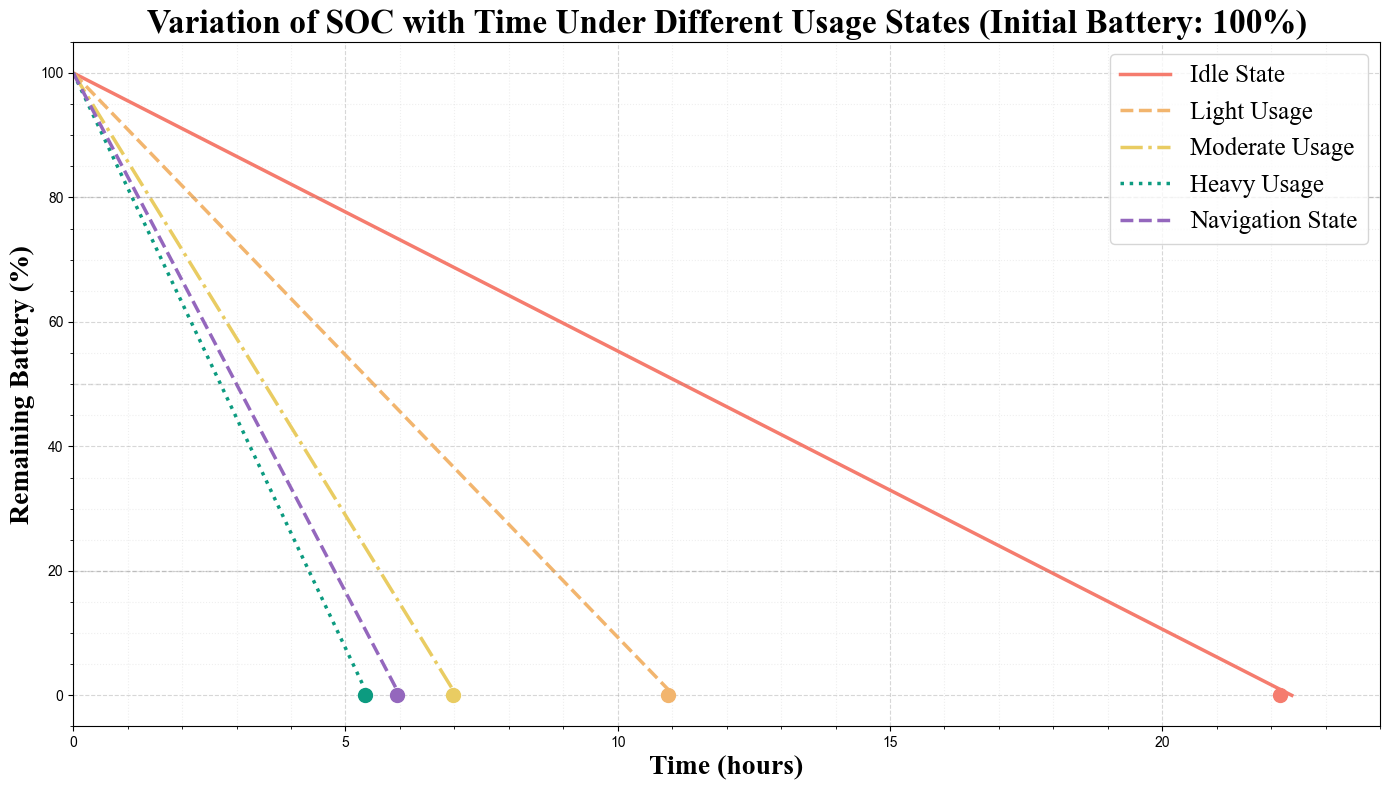
\includegraphics[width=.4\textwidth]{figures/100.png}}%
		\hspace{60pt}
		\subcaptionbox{Discharge Process of Moderate Usage Under Different Initial SOC\label{fig:situation}}%
		{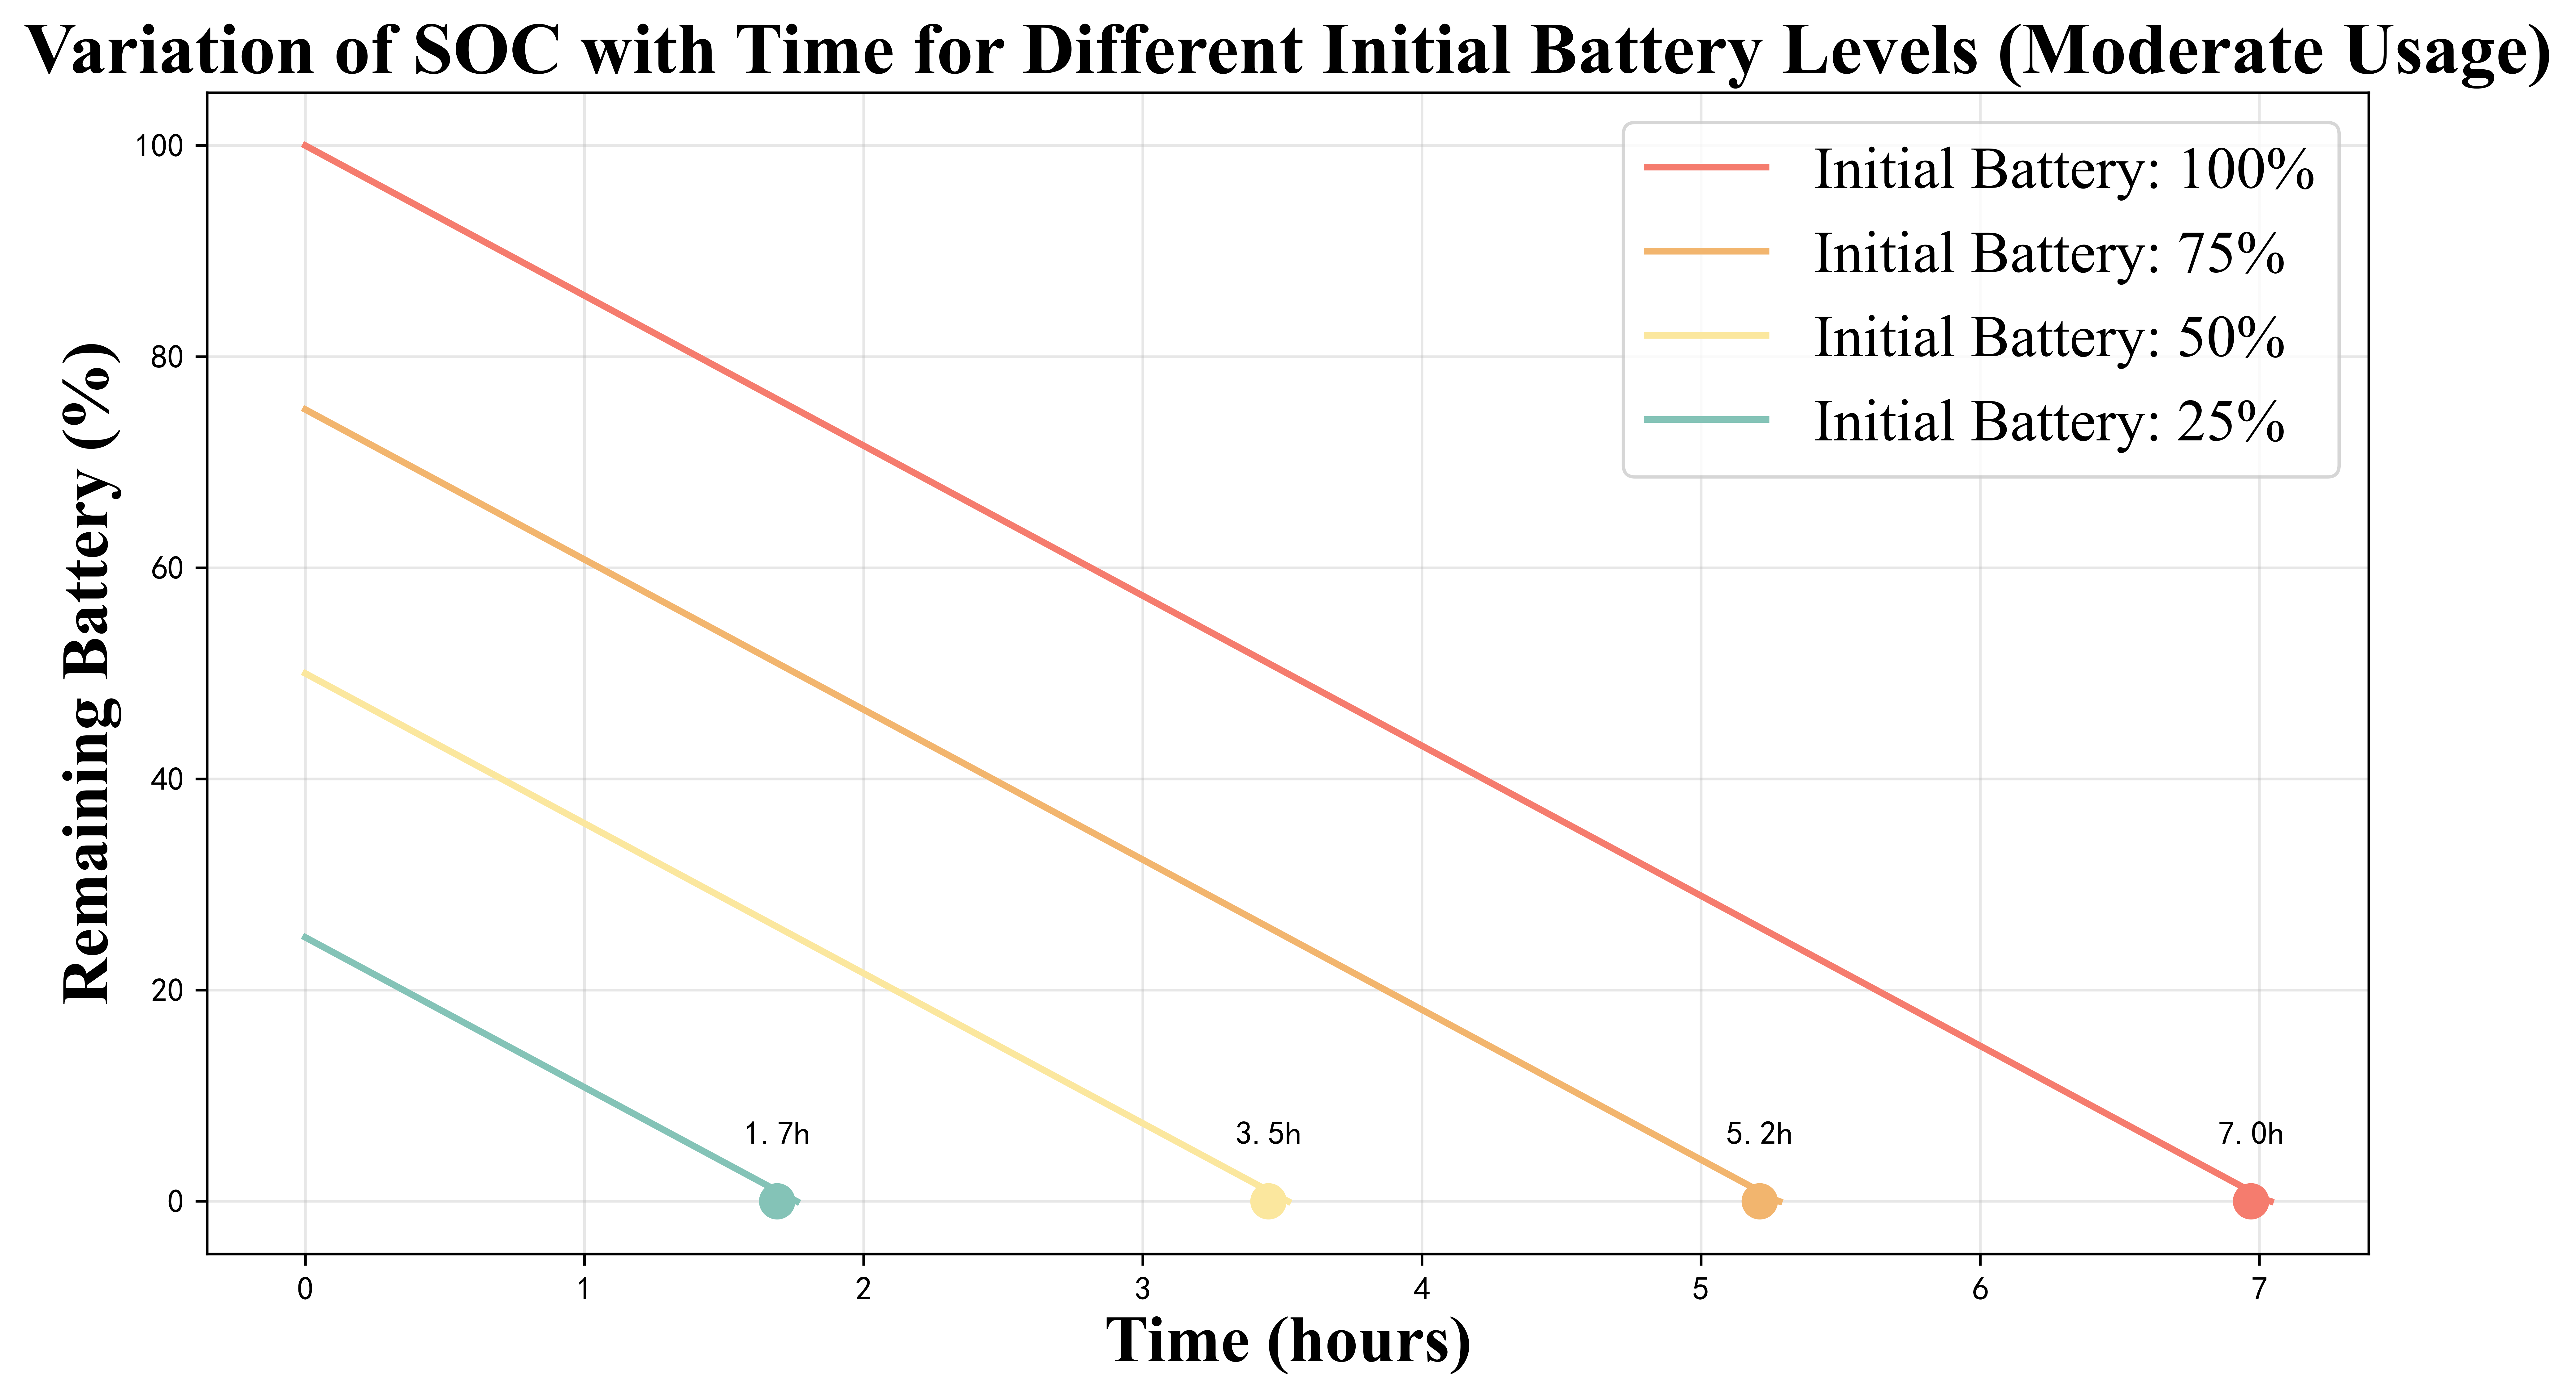
\includegraphics[width=.4\textwidth]{figures/situation.png}}
		\caption{SOC Variation under Different Conditions}
		\renewcommand{\arraystretch}{1.5}
	\end{figure}
	
	\vspace*{-10pt}
	We simulated the SOC variations for each usage scenario under initial charge levels of 100\%, 75\%, 50\%, and 25\%, and calculated the corresponding battery life, as presented in Table 6.
	
	\begin{table}[h!]
		\centering
		\renewcommand{\arraystretch}{1.5}
		\caption{Battery Discharge Duration Under Different Usage States (h)}
		\label{tab:all}
		\begin{tabularx}{0.9\textwidth}{lXXXX} 
			\toprule
			State & 25\% & 50\% & 75\% & 100\% \\
			\midrule
			\rowcolor{LightBlue}
			Idle State & 5.38 & 10.97 & 16.57 & 22.16 \\
			Light Usage & 2.65 & 5.41 & 8.17 & 10.92 \\
			\rowcolor{LightBlue}
			Moderate Usage & 1.69 & 3.45 & 5.21 & 6.97 \\
			Heavy Usage & 1.30 & 2.66 & 4.01 & 5.36 \\
			\rowcolor{LightBlue}
			Navigation State & 1.44 & 2.94 & 4.44 & 5.94 \\
			\bottomrule
		\end{tabularx}
	\end{table}
	
	The power consumption of each module in the smartphone under 5 scenarios is shown in Figure \ref{fig:功率}, and the proportion of each module's power consumption to the total power under the moderate usage scenario is shown in Figure \ref{fig:饼状图}:
	
	\begin{figure}[h!]
		\centering
		\renewcommand{\arraystretch}{0.8}
		\subcaptionbox{Module Power Consumption in Each Scenario\label{fig:功率}}%
		{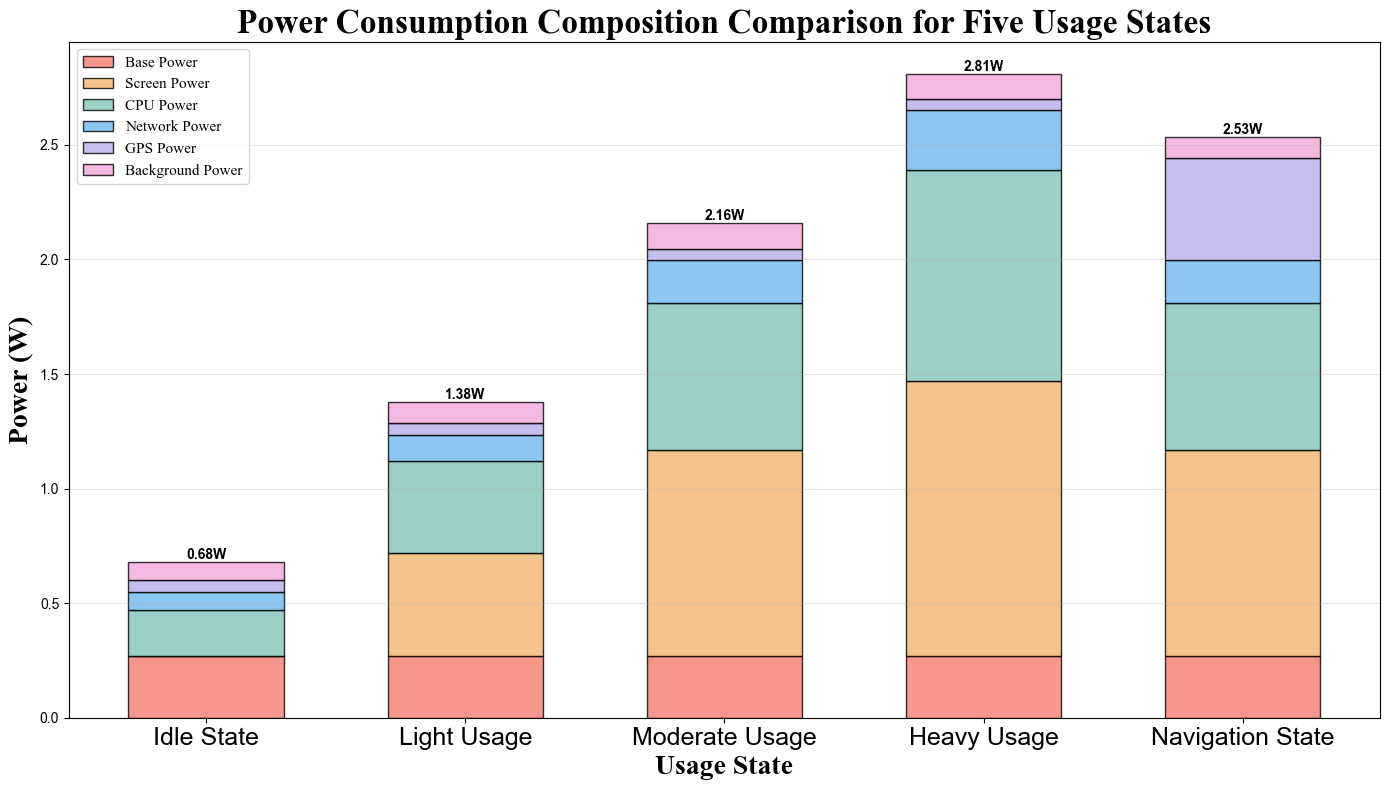
\includegraphics[width=.4\textwidth]{figures/功率.png}}%
		\hspace{60pt}
		\subcaptionbox{Module Power Proportion to Total Power in Moderate Usage\label{fig:饼状图}}
		{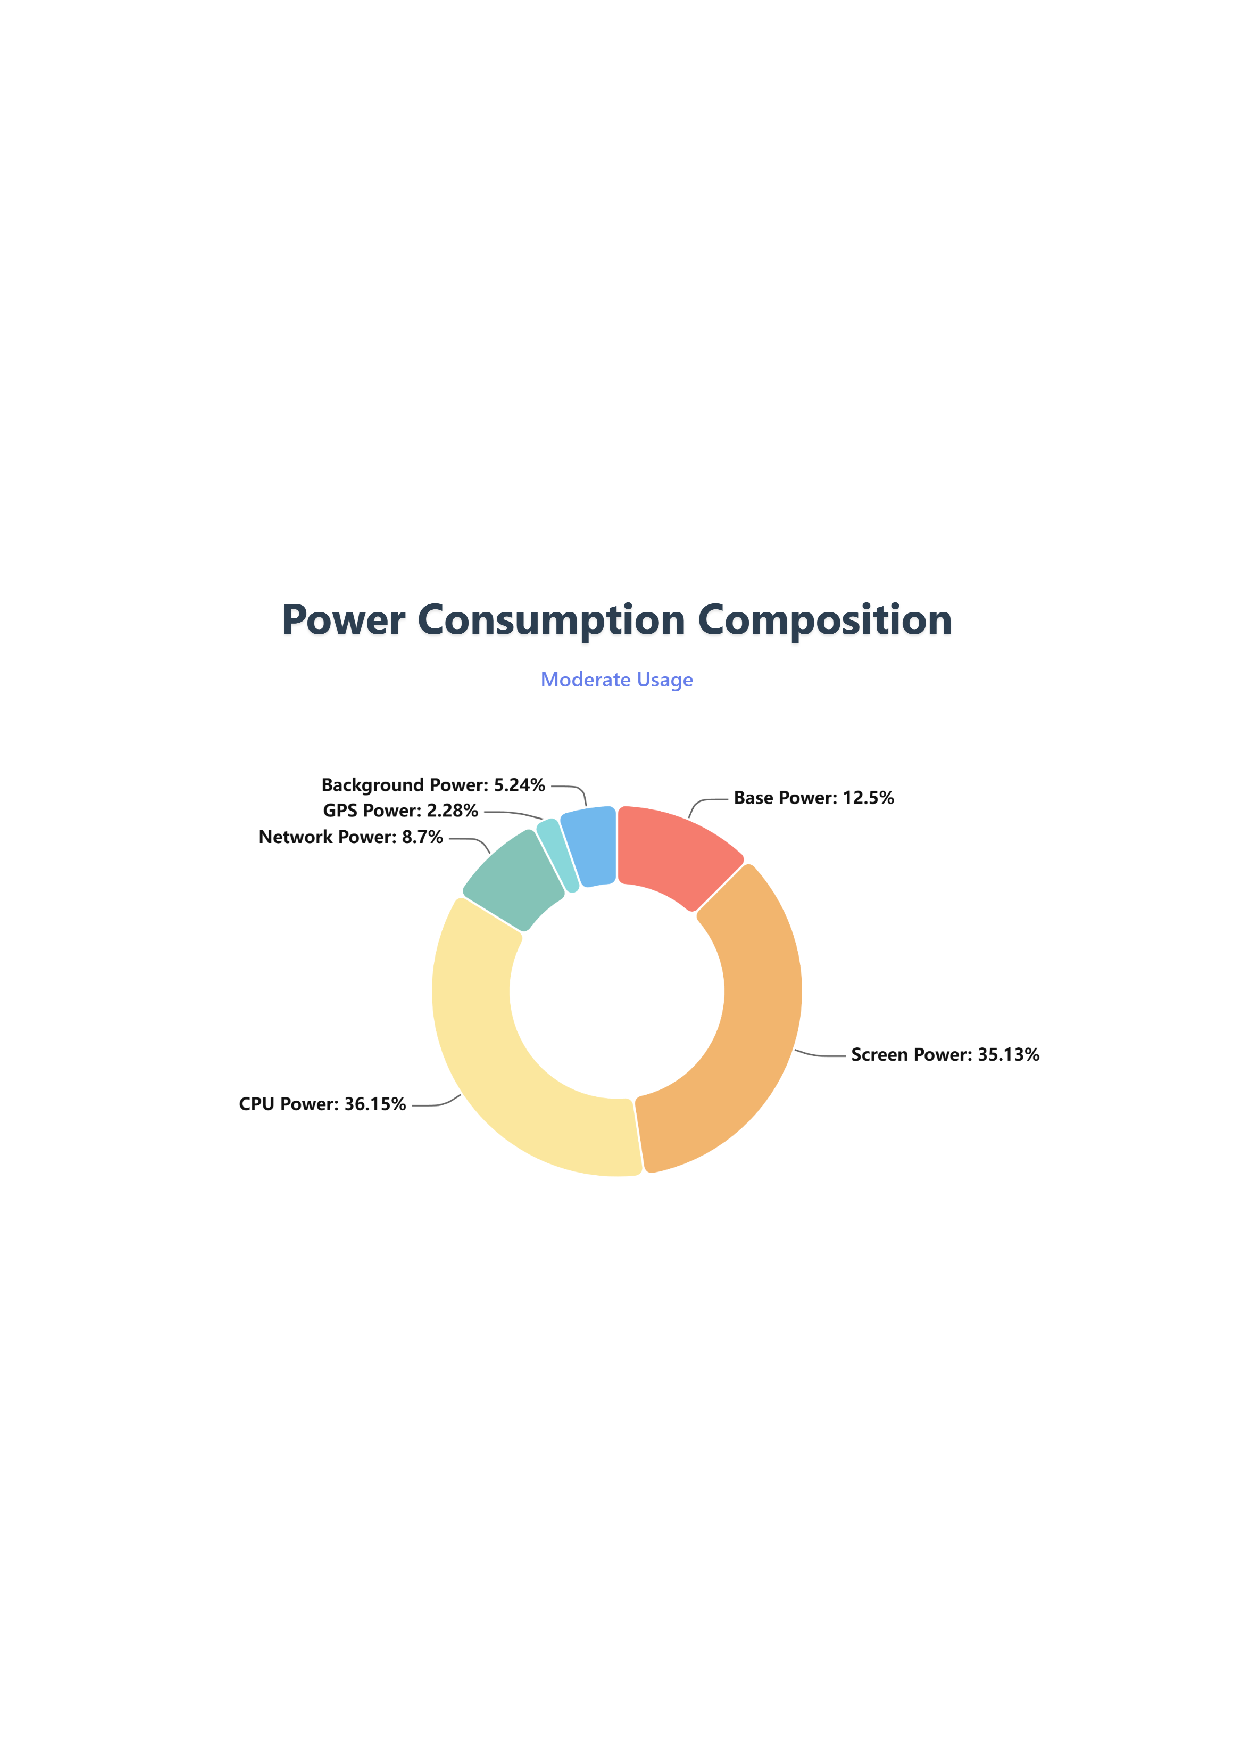
\includegraphics[width=.4\textwidth]{figures/饼状图.pdf}}
		\caption{Power Distribution and Composition}
		\renewcommand{\arraystretch}{1.5}
	\end{figure}
	
	To investigate the influence of each module on smartphone battery discharge, the factors that significantly accelerate the battery discharge rate are analyzed below.
	
	\subsection{Analysis of Significant Influencing Factors}
	To identify the key factors affecting battery life, the control variable method is adopted with the light usage mode as the control group to simulate extreme but realistic usage scenarios. The results show that GPS, CPU load and screen brightness have significant impacts on battery life, while other modules have minor effects:
	In the navigation mode with other modules operating at the light usage level, the average battery life is reduced by 6 hours, a decrease of \textbf{40.354\%};
	At the maximum screen brightness with other modules operating at the light usage level, the average battery life is reduced by 4.85 hours, a decrease of \textbf{32.357\%};
	At the maximum CPU load with other modules operating at the light usage level, the average battery life is reduced by 5.9 hours, a decrease of \textbf{39.575\%}.
	
	\subsection{Uncertainty Quantification Based on the Monte Carlo Method}
	Assuming that variable perturbations follow a normal distribution, the Monte Carlo simulation is used for uncertainty analysis, and uncertainty is quantified by standard deviation, coefficient of variation (CV) and quantile intervals (P5/P95). The coefficient of variation is a dimensionless statistic used to compare the dispersion of different datasets, with the calculation formula as follows:
	\begin{equation}
		CV = \frac{\sigma}{\mu}\times100\%
		\label{eq:cv}
	\end{equation}
	where $\text{CV}$ is the coefficient of variation, $\sigma$ is the population standard deviation, and $\mu$ is the population mean. A smaller CV value indicates lower relative volatility and more concentrated data. The results of the uncertainty analysis are shown in Table \ref{tab:控制变量}.
	
	\begin{table}[h!]
		\centering
		\renewcommand{\arraystretch}{1.5}
		\caption{Uncertainty Analysis Results Under Different Scenarios}
		\label{tab:控制变量}
		\begin{tabular}{lccccc}
			\toprule
			Scenario & Mean (h) & Standard Deviation (h) & CV & P5 (h) & P95 (h) \\
			\midrule
			\rowcolor{LightBlue}
			Low Load-Positioning-10℃ & 15.9291 & 0.6611 & 0.0415 & 14.8889 & 16.9940 \\
			Low Load-Positioning-25℃ & 14.9978 & 0.6667 & 0.0445 & 13.9795 & 16.2103 \\
			\rowcolor{LightBlue}
			Low Load-Positioning-40℃ & 14.1443 & 0.6233 & 0.0441 & 13.1096 & 15.2563 \\
			Navigation-10℃ & 10.9844 & 0.3324 & 0.0303 & 10.4562 & 11.5742 \\
			\rowcolor{LightBlue}
			Navigation-25℃ & 10.3858 & 0.3037 & 0.0292 & 9.8866 & 10.8728 \\
			Navigation-40℃ & 9.7356 & 0.3018 & 0.0310 & 9.2585 & 10.2374 \\
			\rowcolor{LightBlue}
			High Brightness-10℃ & 10.7639 & 0.4516 & 0.0420 & 10.0645 & 11.5598 \\
			High Brightness-25℃ & 10.1574 & 0.4142 & 0.0408 & 9.4838 & 10.8397 \\
			\rowcolor{LightBlue}
			High Brightness-40℃ & 9.5467 & 0.3822 & 0.0400 & 8.9356 & 10.2018 \\
			High CPU-10℃ & 9.6149 & 0.2417 & 0.0251 & 9.2173 & 10.0310 \\
			\rowcolor{LightBlue}
			High CPU-25℃ & 9.0821 & 0.2341 & 0.0258 & 8.7323 & 9.4651 \\
			High CPU-40℃ & 8.5487 & 0.2310 & 0.0270 & 8.2051 & 8.9518 \\
			\bottomrule
		\end{tabular}
	\end{table}
	
	It can be seen from Table \ref{tab:控制变量} that the model has a small coefficient of variation under all scenarios, indicating low uncertainty and high stability of the model. Relatively, the average coefficient of variation (0.04) in the scenarios of navigation, high CPU and high network load is slightly higher than that (0.03) in the scenarios of high CPU and navigation.
	
	
	\section{Rationality of Assumptions and Sensitivity of Parameters}
	
	To evaluate the robustness and reliability of the proposed model, we conduct a comprehensive sensitivity analysis by systematically modifying key assumptions, introducing parameter perturbations, and varying usage patterns, thereby assessing their impact on prediction outcomes.
	
	\subsection{Sensitivity to Model Assumptions}
	
	We examine the reasonableness of two fundamental assumptions: screen type selection and constant temperature conditions. By altering these assumptions individually, we analyze their influence on model performance.
	
	\subsubsection{Variation in Screen Type Assumption}
	
	To assess the model's adaptability to different display technologies, we replace the original OLED screen assumption with an LCD screen. Under this modified assumption, we repeat the random simulation under identical experimental conditions:
	\begin{figure}[h!]
		\centering
		\renewcommand{\arraystretch}{1}
		\subcaptionbox{Random simulation of synchronized parameter changes in LCD screens\label{fig:同步变化的随机仿真第三问}}%
		{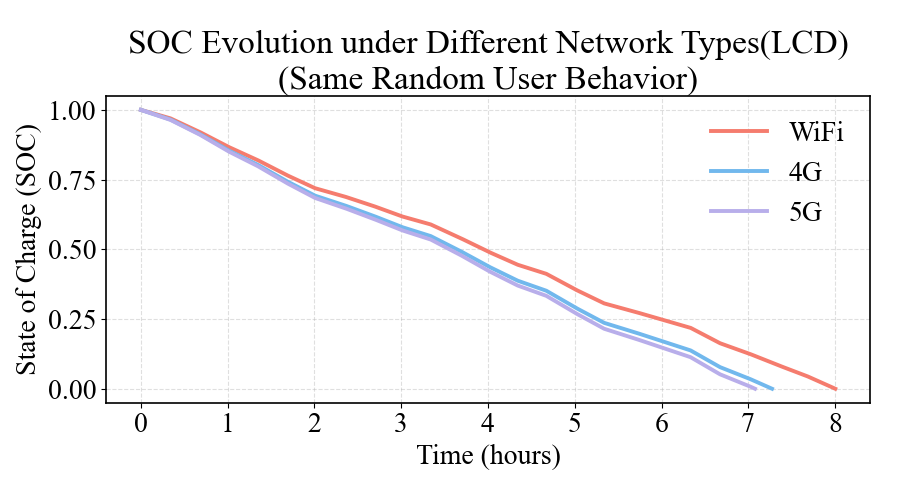
\includegraphics[width=.4\textwidth]{figures/同步变化的随机仿真第三问.png}}%
		\hspace{60pt}
		\subcaptionbox{Random simulation of independent parameter changes in LCD screens\label{fig:独立变化的随机仿真第三问}}
		{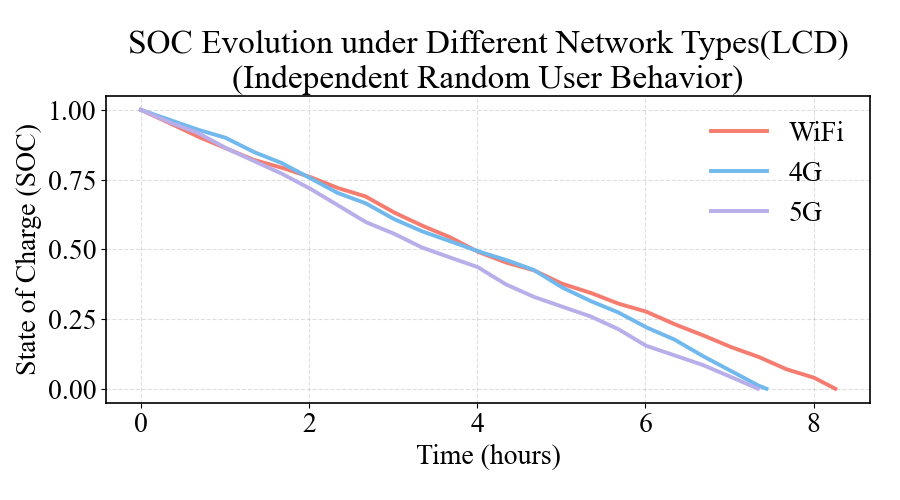
\includegraphics[width=.4\textwidth]{figures/独立变化的随机仿真第三问.png}}
		\caption{Random simulation using LCD screen}
		\renewcommand{\arraystretch}{1.5}
	\end{figure}
	
	
	\begin{table}[h!]
		\centering
		\caption{Random simulation of synchronized parameter changes data(LCD)}
		\label{tab:LCD屏同步变化的随机仿真第三问}
		\renewcommand{\arraystretch}{1.5}
		\begin{tabularx}{0.8\textwidth}{lXXX} 
			\toprule
			\textbf{指标} & \textbf{Wi-Fi} & \textbf{4G} & \textbf{5G} \\
			\midrule
			\rowcolor{LightGreen}
			总放电时间 (h) & 8.00 & 7.27 & 7.08 \\
			平均SOC衰减速率 (h$^{-1}$) & 0.1250 & 0.1375 & 0.1413 \\
			\rowcolor{LightGreen}
			50\% SOC放电时间 (h) & 3.95 & 3.64 & 3.56 \\
			\bottomrule
		\end{tabularx}
	\end{table}
	
	\begin{table}[h!]
		\centering
		\caption{Random simulation of independent parameter changes data(LCD)}
		\label{tab:LCD屏独立变化的随机仿真第三问}
		\renewcommand{\arraystretch}{1.5}
		\begin{tabularx}{0.8\textwidth}{lXXX}
			\toprule
			\textbf{指标} & \textbf{Wi-Fi} & \textbf{4G} & \textbf{5G} \\
			\midrule
			\rowcolor{LightGreen}
			总放电时间 (h) & 8.26 & 7.44 & 7.34 \\
			平均SOC衰减速率 (h$^{-1}$) & 0.1211 & 0.1344 & 0.1363 \\
			\rowcolor{LightGreen}
			50\% SOC放电时间 (h) & 3.95 & 3.94 & 3.40 \\
			\bottomrule
		\end{tabularx}
	\end{table}
	
	\newpage
	The characteristics of the three network types derived from the corresponding charts and tables are consistent with those obtained from random simulations using an OLED screen, indicating that the model has wide adaptability to screen types.
	\subsubsection{Variation in Constant Temperature Assumption}
	We introduce a differential equation to reflect the power-thermal feedback situation:
	\begin{equation}
		C_T \frac{dT}{dt} = \eta P_{\text{total}} - h(T - T_{\text{amb}})
	\end{equation}
	where $C_T$ is the device's thermal capacity, common range is $4 \sim 8\ \mathrm{J}/^\circ\mathrm{C}$; $\eta$ is the power-to-heat conversion efficiency, common range is $0.9 \sim 1.0$; $h$ is the heat transfer coefficient, common range is $2\sim16\ s$. Under moderate usage, the random simulation results of the thermal feedback model and the constant temperature model are shown in Figure \ref{fig:考虑热反馈一致}.
	
	\begin{figure}[h!]
		\centering
		\vspace*{-10pt}
		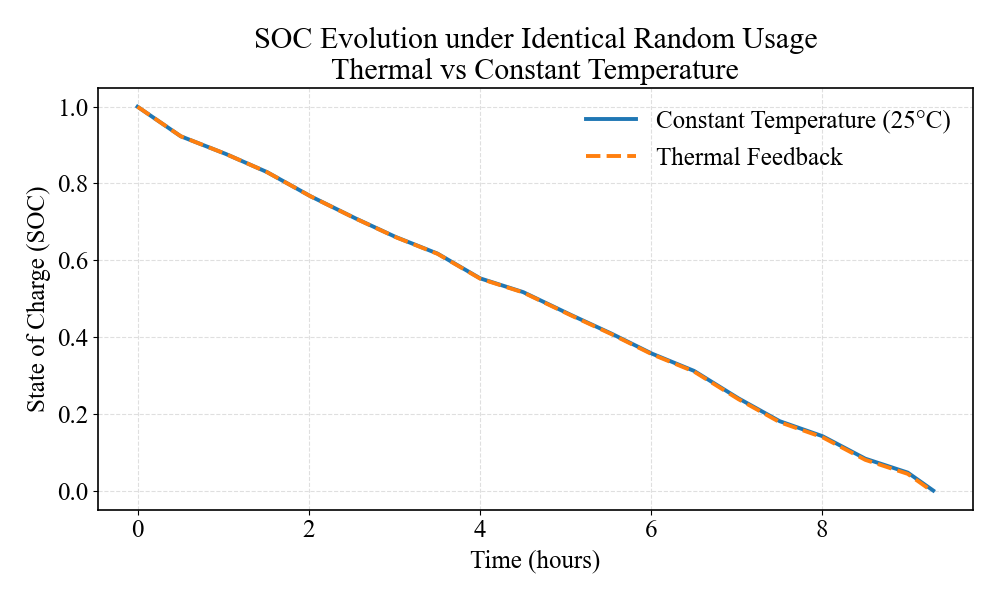
\includegraphics[width=0.5\textwidth,trim=0cm 0.4cm 0cm 0cm,clip]{figures/考虑热反馈一致.png}
		\caption{Thermal feedback vs. constant temperature model}
		\label{fig:考虑热反馈一致}
	\end{figure}
	
	The results show that under high load and high ambient temperature conditions, thermal feedback can further shorten battery life and amplify the uncertainty caused by input disturbances. However, the sensitivity ranking of key usage parameters (CPU load, network activity, and screen brightness) remains consistent before and after introducing thermal feedback. The battery life of the constant temperature model is 9.30 hours, and that of the thermal feedback model is 9.28 hours, a change of only \textbf{0.02 hours}, with a magnitude of only \textbf{0.25\%}, indicating that the model has strong robustness to assumption changes.
	
	\subsection{Sensitivity Analysis}
	\subsubsection{Sensitivity of Parameter values}
	We introduce \textbf{Standardized Regression Coefficient (SRC)} to reflect the parameter sensitivity of the model:
	\begin{equation}
		\mathrm{SRC}_i = \beta_i \frac{\sigma_{X_i}}{\sigma_Y},
	\end{equation}
	where $\sigma_{X_i}$ and $\sigma_Y$ are the standard deviations of parameter $X_i$ and output $Y$, respectively.
	The absolute value of SRC reflects the relative intensity of a parameter's influence on the model output; the larger the value, the stronger the sensitivity.
	
	\begin{table}[htbp]
		\centering
		\caption{SRC values of each variable}
		\renewcommand{\arraystretch}{0.8}
		\begin{tabular}{@{}ccccccccccc@{}}
			\toprule
			Variable & $u$ & $B$ & $a_{cpu}$  & $\beta$ & $r$ & $\alpha$  & $a_{wifi}$ & $bg$ & $\gamma$ & $\phi_T$ \\
			\midrule
			\rowcolor{LightBlue}
			SRC & -0.595 & -0.492 & -0.476  & -0.195 & -0.136 & -0.125 & -0.114 & -0.070 & -0.033 & 0.001 \\
			\bottomrule
		\end{tabular}
		\label{tab:src}
	\end{table}
	
	From Table \ref{tab:src}, the parameters sensitive to parameter values are CPU load ($u$, SRC=-0.595) and screen brightness ($B$, SRC=-0.492). Increasing CPU load from 40\% to 90\% can shorten discharge time by about 38\%. The parameters with moderate sensitivity are the network and screen coefficients and CPU coefficients ($a_{\text{cpu}}$, $b_{\text{cpu}}$); a 10\% error in these can cause about a 4.8\% deviation in discharge time prediction. The parameters with weak sensitivity are the temperature coefficient ($\phi_T$, SRC=+0.001), whose impact on power consumption is negligible at room temperature, consistent with previous analysis results.
	
	Since SRC is based on regression analysis, correlations between parameters may lead to bias in sensitivity estimates. Therefore, we further introduce the Variance Inflation Factor (VIF) to test for multicollinearity:
	
	\vspace*{-15pt}
	\begin{equation}
		\mathrm{VIF}_i = \frac{1}{1 - R_i^2}
	\end{equation}
	where $R_i^2$ is the coefficient of determination obtained by regressing $X_i$ on the other input parameters.
	
	\begin{table}[htbp]
		\centering
		\hspace*{-40pt}
		\caption{VIF values of each variable}
		\renewcommand{\arraystretch}{0.8}
		\begin{tabular}{@{}ccccccccccc@{}}
			\toprule
			Variable & $\alpha$ & $\beta$ & $\gamma$ & $a_{cpu}$ & $a_{wifi}$ & $\phi_T$ & $B$ & $u$ & $r$ & $bg$ \\
			\midrule
			\rowcolor{LightBlue}
			VIF & 1.013 & 1.024 & 1.017 & 1.016 & 1.016 & 1.014 & 1.007 & 1.011 & 1.008 & 1.013  \\
			\bottomrule
		\end{tabular}
		\label{tab:vif}
	\end{table}
	
	The calculation results show that the VIF values of all major parameters are within the common threshold range, with no significant multicollinearity, indicating that the sensitivity ranking reflected by SRC is stable and reliable.
	
	Subsequently, we simultaneously perturb 12 parameters. The statistical \textbf{CV value} is about 5.52\%, and the relative fluctuation of discharge time remains at a low level, indicating the model has strong stability.
	
	\begin{table}[htbp]
		\centering
		\caption{Uncertainty Quantification Metrics}
		\renewcommand{\arraystretch}{0.8}
		\begin{tabular}{@{}ccccc@{}}
			\toprule
			Mean Time (h) & Std Dev (h) & CV & P5 (h) & P95 (h) \\
			\midrule
			\rowcolor{LightBlue}
			12.422 & 0.685 & 0.055 & 11.372 & 13.532 \\
			\bottomrule
		\end{tabular}
		\label{tab:CV}
	\end{table}
	
	\vspace*{-10pt}
	\subsubsection{Changing fluctuations in usage patterns}
	We validate the model's robustness by changing the frequency of usage scenario switches. We set a base sequence with 2000 behavior points at 1-minute intervals and control all variation groups to share the same base behavior sequence for scenario changes to achieve synchronized changes. The random simulation results are shown in Figure \ref{fig:波动}.
	\begin{figure}[h!]
		\centering
		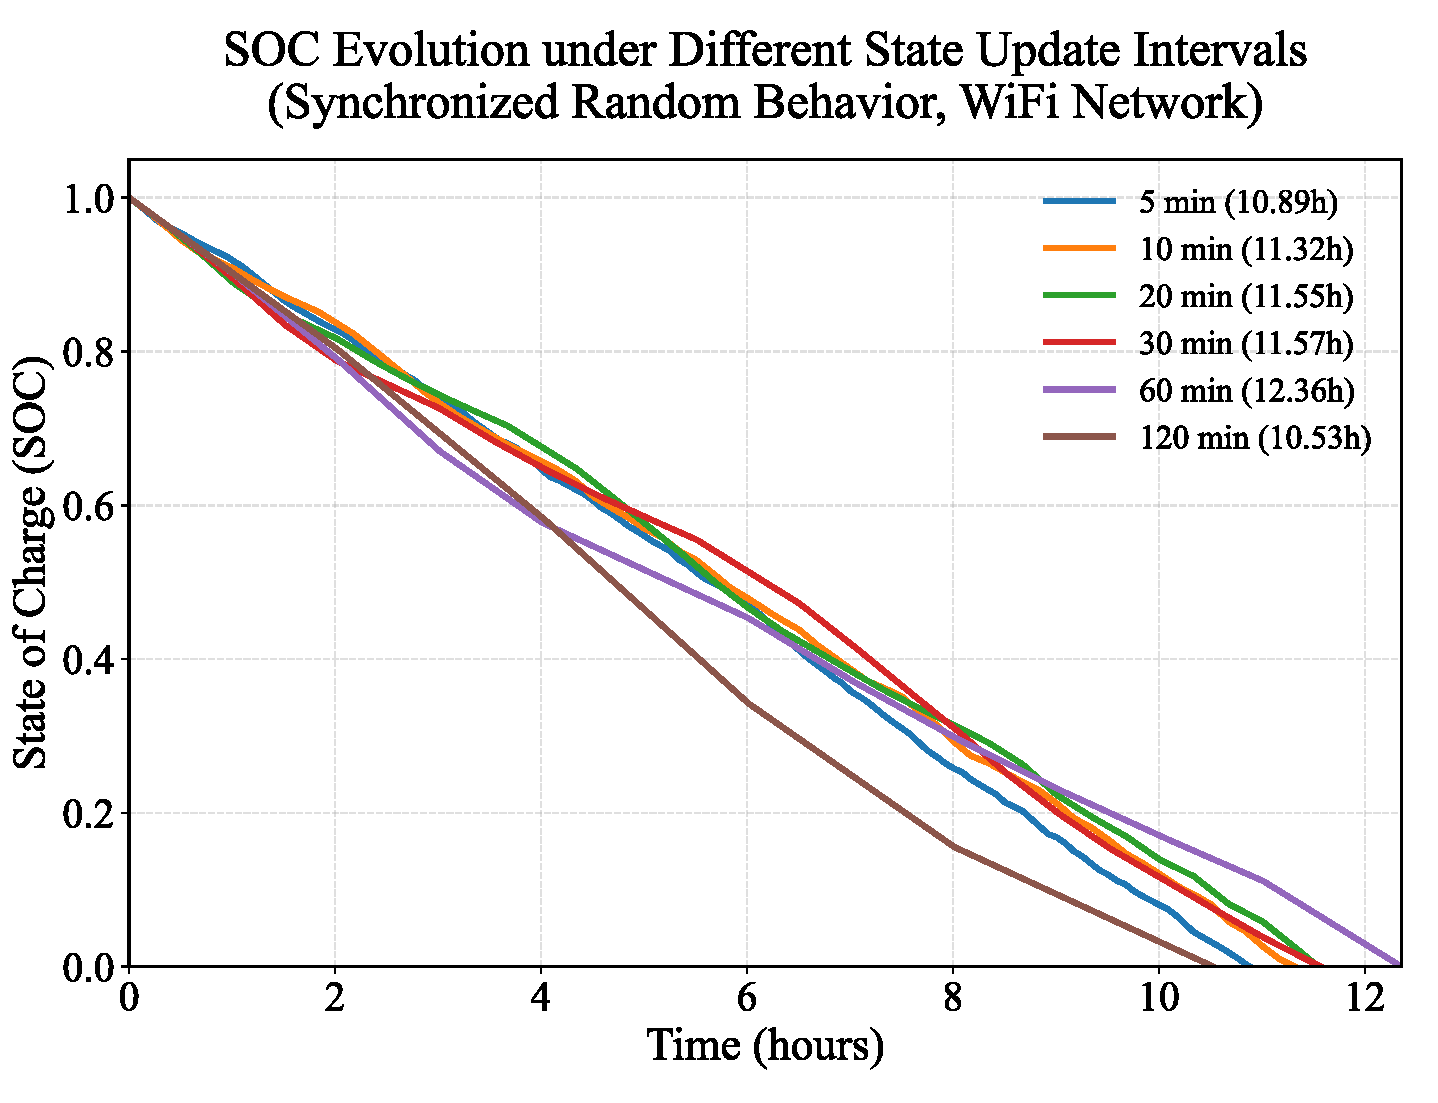
\includegraphics[width=0.5\textwidth,trim=0cm 0.4cm 0cm 0cm,clip]{figures/波动.pdf}
		\caption{Random simulation results under different switching frequencies}
		\label{fig:波动}
	\end{figure}
	
	According to the experimental results, the optimal update interval for the device is 60 minutes, at which point the battery life can reach up to 12.36 hours. The worst update interval is 120 minutes, corresponding to a battery life of 10.53 hours, a difference of 1.83 hours (17.4\%). Frequent updates lead to rapid device behavior changes, large power consumption fluctuations, and lower battery efficiency. Moderate updates result in relatively stable behavior changes and power consumption, leading to higher battery efficiency. Sparse updates may cause slow behavior changes and prolonged periods of unfavorable power consumption states. Therefore, in practical applications, an update interval strategy of about 60 minutes is recommended to maximize battery life, offering a 17.4\% improvement compared to the worst-case scenario.
	
	
	
	
	\section{Recommendations}  % 一级标题
	
	\subsection{Recommendations for Smartphone Users}
	
	
	\begin{enumerate}[label=\bfseries\arabic*.]
		\item \textbf{On-demand activation of core power-consuming modules}: GPS activation reduces battery life by up to 40.354\%, full CPU load reduces it by 39.575\%, and maximum screen brightness reduces it by 32.357\%. It is recommended to turn off GPS when not navigating, close high-load background applications, and adjust screen brightness to around 30\%.
		
		\item \textbf{Avoid maintaining the phone in high-performance mode}: Standby mode achieves the longest battery life of 22.16h, while heavy usage only lasts 5.36h and navigation 5.94h. Switch to standby promptly when not in use, and reduce the duration of heavy or navigation scenarios.
		
		\item \textbf{Avoid combining high-temperature and high-load usage}: At $40^\circ$\text{C}, battery life in various high-power scenarios decreases by 8\%-12\% compared to $10^\circ\mathrm{C}$. Avoid simultaneous use of navigation, high brightness, and high-load functions in high-temperature environments.
		
		\item \textbf{Optimize the frequency of usage behavior switching}: Adjust usage behavior every 60 minutes for optimal battery life (up to 12.36h). Avoid fixed high-power usage exceeding 120 minutes (battery life drops to 10.53h, a reduction of 17.4\%).
		
		\item \textbf{Prioritize Wi‑Fi in static usage scenarios}: For phones equipped with OLED screens, Wi‑Fi provides a battery life of 10.66 h, while 5G lasts only 9.18 h. It is therefore recommended to turn off unnecessary 4G or 5G network connections.
	\end{enumerate}
	
	
	\subsection{Recommendations for Operating Systems}
	
	
	\begin{enumerate}[label=\arabic*.]
		\item \textbf{Fine-grained Control of Core Sensitive Parameters}: CPU load (SRC = -0.595) and screen brightness (SRC = -0.492) are the most sensitive parameters. Real-time dynamic adjustment can reduce 4.8\% of the battery life prediction error by lowering parameter errors by 10\%.
		\item \textbf{Scenario-aware intelligent power scheduling:} Automatically identify five types of usage scenarios and match them with preset power parameters. Limit non-core CPU load in navigation scenarios and cap screen brightness in light usage scenarios. The default scenario update interval is 60 minutes.
		\item \textbf{Temperature-Adaptive Power Limitation}: When the device temperature approaches $40^\circ\mathrm{C}$, proactively limit functions such as GPS, high brightness, and high CPU load to avoid battery life degradation caused by thermal feedback.
		\item \textbf{Low-Uncertainty Battery Life Prediction}: To ensure prediction stability, parameters with a CV < 0.045 were selected for modeling. Ignore the interference of the temperature coefficient (SRC = 0.001) under normal temperature to accurately indicate the remaining battery life.
		\item \textbf{Intelligent Network Mode Switching}: Compared with 5G, Wi‑Fi extends battery life by 12.5\%. When the Wi‑Fi signal is stable, the device should automatically switch from 4G or 5G to Wi‑Fi to mitigate the power surge caused by network switching.
	\end{enumerate}
	
	
	\subsection{Recommendations Considering Battery Aging}
	
	
	Battery aging is primarily caused by calendar aging and cycle aging: calendar aging manifests as the performance degradation of the battery over time while in a static state, and cycle aging results from cumulative damage caused by repeated charge and discharge cycles during usage. Together, these two mechanisms lead to battery capacity fade and increased internal resistance. Considering measurement convenience and direct relevance to user experience, we choose to establish an aging model from the perspective of battery capacity.
	
	\begin{equation}
		\begin{cases}
			C(t) = C_0\bigl(1 - \lambda_1 t - \lambda_2 n(t)\bigr) \\[8pt]
			C_{\text{avail}}(t) = C_{\text{eff}}(t) \left(1 - \gamma \dfrac{P_{\text{total}}(t)}{P_{\text{ref}}}\right)
		\end{cases}
	\end{equation}
	where $C(t)$ is the actual available battery capacity at time $t$, $C_0$ is the initial rated capacity, $\lambda_1$ and $\lambda_2$ are the calendar and cycle aging coefficients with empirical ranges $\lambda_1\in [0.01,0.05]$ \upcite{9} and $\lambda_2\in [10^{-4},10^{-3}]$ \upcite{10} respectively, $n(t)$ is the cumulative number of charge-discharge cycles, $C_{\text{avail}}(t)$ is the capacity under current load, $C_{\text{eff}}(t)$ is the effective capacity after aging corrections, $\gamma$ is the internal resistance–load sensitivity coefficient ($\gamma\in [0.05,0.2]$ \upcite{11}), $P_{\text{total}}(t)$ is the total device power consumption, and $P_{\text{ref}}$ is a reference power. From this, we derive the differential equation for state of charge (SOC) evolution considering battery aging:
	
	\begin{equation}
		\frac{d \left(\text{SOC}(t)\right)}{dt} = - \frac{P_{\text{total}}(t)}{C_0 \cdot \bigl(1 - \lambda_1 t - \lambda_2 n(t)\bigr) \cdot V \cdot \Phi(T) \cdot \left(1 - \gamma \frac{P_{\text{total}}(t)}{P_{\text{ref}}}\right)}
	\end{equation}
	
	Considering the impact of battery aging on battery life, we recommend that users maintain the charge level between 50\% and 80\% during long-term storage of smartphone and check the charge every three months; during daily use, try to keep the charge within 20\%-80\%, avoiding deep discharges and prolonged full-charge states; if the battery exhibits significantly reduced runtime, abnormal heating, or physical swelling, it should be inspected or replaced promptly. At the same time, we recommend that manufacturers integrate battery health monitoring features and alert users when health drops below 80\%, prompting battery or device replacement.
	
	\subsection{Model Expansion}
	
	We select smart bands for model extension, as their battery life is also influenced by user behavior\upcite{12}. By appropriately recalibrating key parameters, the model can be thereby adapted to their characteristics of smaller battery capacity and lower computational load. The simulation results match the actual discharge data, indicating the model's potential for broader application.
	
	\begin{figure}[h!]
		\centering
		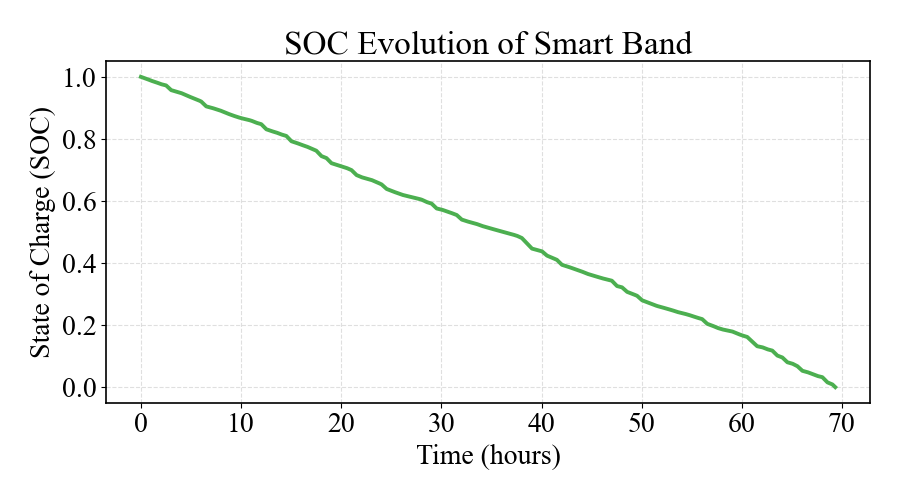
\includegraphics[width=0.5\textwidth,trim=0cm 0.4cm 0cm 0cm,clip]{figures/手环.png}
		\caption{Application of the Model to Smart Watch}
		\label{fig:手环}
	\end{figure}
	
	\vspace*{-14pt}
	\section{Model Evaluation}  % 一级标题
	
	\subsection{Strengths}
	\begin{itemize}
		\item \textbf{Reliability of Model Structure:} We adopt a continuous-time differential equation framework for SOC, with total power consumption as its driving term. Avoiding sophisticated battery internal principles, the model is simplified yet with sound structural reliability and physical rationality. 
		\item \textbf{Scientificity of Parameter Selection:} All key parameters in the model, including power consumption coefficients and battery aging coefficients, are determined by referring to valid ranges in academic literatures and authoritative measurement reports, ensuring the scientificity and practical applicability of the model.
		\item \textbf{Rationality of Data Application:} The data adopted in this paper is mainly used to verify the rationality of power consumption and the accuracy of parameter values, rather than for fitting or regression analysis of the SOC time series. 
		\item \textbf{Generalizability of the Model:} The model applies to multiple portable electronics, such as smart bracelets, tablets and laptops. Targeted adjustment of core parameters enables its adaptation to diverse device hardware and scenarios.
	\end{itemize}
	
	\vspace*{-10pt}
	\subsection{Weaknesses}
	\begin{itemize}
		\item \textbf{Insufficiency of Verification Data:} The model verification mainly relies on public datasets such as academic literatures, industry reports and published test data, lacking further verification with large-scale and multi-dimensional measured data from real scenarios. 
		\item \textbf{Limitations in Refined Scenario Simulation:} Although the model covers core differences via stochastic simulation and parameterization, it can hardly characterize App background heterogeneity, hardware specificity, or real users’ fragmented usage behaviors in detail.
	\end{itemize}
	
	
	

	
	
	
	\newpage
	\phantomsection  % 创建锚点
	\addcontentsline{toc}{section}{References}
	\begin{thebibliography}{99}%宽度9
	\bibitem{1} CARROLL A, HEISER G. An Analysis of Power Consumption in a Smartphone[C]//Proc. 2010 USENIX conf., USENIX Assoc. 2010.
	\bibitem{2} Dash, P., \& Hu, Y. C. (2021). How much battery does dark mode save? An accurate OLED display power profiler for modern smartphones. In \textit{Proceedings of the 19th Annual International Conference on Mobile Systems, Applications, and Services} (pp. 1–13). ACM. https://doi.org/10.1145/3458864.3467682
	\bibitem{3} DONG M, CHOI Y S K, ZHONG L. Power modeling of graphical user interfaces on OLED displays[C/OL]//2009 46th ACM/IEEE Design Automation Conference. 2009: 652-657[2026-01-31]. https://ieeexplore.ieee.org/document/5227097.
	\bibitem{4} CHOI Y, HA R, CHA H. Fully automated OLED display power modeling for mobile devices[J/OL]. Pervasive and Mobile Computing, 2018, 50: 41-55. DOI:10.1016/j.pmcj.2018.07.006.
	\bibitem{5} R. Cheng, J. Lu, H. Jiang, et al., "Research on energy consumption model of intelligent mobile terminals," *Computer Technology and Development*, vol. 27, no. 12, pp. 128-132, 138, Dec. 2017.
	\bibitem{6} Gupta, A., Heidari, A., Kalipattapu, A., et al. (2024). 3 W’s of smartphone power consumption: Who, Where and How much is draining my battery? In \textit{Proceedings of the 30th Annual International Conference on Mobile Computing and Networking} (pp. 2248–2250). Association for Computing Machinery. https://doi.org/10.1145/3636534.3695905
	\bibitem{7}Kim J H, Lee S J, Kim Y J. Temperature-dependent performance of smartphone batteries[J]. IEEE Transactions on Consumer Electronics, 2015, 61(3): 292-298.
	\bibitem{8}Huang, X. H., \& Hu, Z. H. (2012). A brief analysis of the Runge-Kutta method. *Heilongjiang Science and Technology Information*, (23), 28.
	\bibitem{9}Ali, H., Beltran, H., Lindsey, N. J., \& Pecht, M. (2023). Assessment of the calendar aging of lithium-ion batteries for a long-term—Space missions. Frontiers in Energy Research, 11. https://doi.org/10.3389/fenrg.2023.1108269
	\bibitem{10}Gantenbein, S., Schönleber, M., Weiss, M., \& Ivers-Tiffée, E. (2019). Capacity Fade in Lithium-Ion Batteries and Cyclic Aging over Various State-of-Charge Ranges. Sustainability, 11(23), 6697. https://doi.org/10.3390/su11236697
	\bibitem{11}Li, W., Zhang, H., van Vlijmen, B., Dechent, P., \& Sauer, D. U. (2021). Forecasting battery capacity and power degradation with multi-task learning [Preprint]. arXiv. https://arxiv.org/abs/2111.14937
	\bibitem{12}Sunder, R., Lilhore, U. K., Rai, A. K., et al. (2025). SmartAPM framework for adaptive power management in wearable devices using deep reinforcement learning. *Scientific Reports*, *15*, 6911. https://doi.org/10.1038/s41598-025-89709-3
	\end{thebibliography}
	
	%%%%%%%%%%%%%%%%%%%%%%% 正文结束 %%%%%%%%%%%%%%%%%%%%%%%
	
	\newpage
	\section*{\centering Report on Use of AI Tools}
	
	\subsection*{1. OpenAI ChatGPT (Feb 2, 2026 version, GPT-5.2)}
	\begin{itemize}
		\item \textbf{Query}: Could you please provide relevant literature and links on mobile phone power consumption, so that we can examine the parameters of our established model?
		\item \textbf{Output}: Here are some important academic papers on smartphone power (energy) modeling, analysis, and optimization, along with accessible links, which are suitable for building, validating, or comparing parameters of power models:
		\begin{enumerate}[label=(\arabic*)]
			\item \textit{Modeling of Smartphones Power Using Neural Networks} — Uses neural networks to build a smartphone power prediction model, analyzing the relationship between user behavior and power consumption.
			\item \textit{The Influence of Temperature on the Capacity of Lithium Ion Batteries with Different Anodes} — This study can be used to analyze the impact of temperature on smartphone battery performance, with relevant parameters available.
			\item \textit{An Analysis of Power Consumption in a Smartphone} — This seminal research provides a comprehensive analysis of various factors affecting power consumption in smartphones, which can be referenced.
		\end{enumerate}
	\end{itemize}
	
	\subsection*{2. OpenAI ChatGPT (Feb 2, 2026 version, GPT-5.2)}
	\begin{itemize}
		\item \textbf{Query}: What are the key concepts related to the Standardized Regression Coefficient (SRC) and the Coefficient of Variation (CV)?
		\item \textbf{Output}: Both SRC and CV are tools that use standardization to eliminate differences in units, but they serve different purposes: SRC is used in regression analysis to fairly compare the influence of different variables on an outcome, while CV is used in descriptive statistics to compare the variability (or stability) between different datasets. In simple terms, SRC compares the impact of variables, whereas CV compares the stability of the data itself.
	\end{itemize}
	
	\subsection*{3. OpenAI ChatGPT (Feb 2, 2026 version, GPT-5.2)}
	\begin{itemize}
		\item \textbf{Query}: What is the technical principle of stochastic simulation?
		\item \textbf{Output}: The fundamental principle of random state switching simulation is to abstract the system into several discrete states. It assumes that the system remains in a given state for a random duration and then switches to another state according to specified transition probabilities. Both the dwell time and state transitions are determined by random variables, typically implemented by generating uniform random numbers and sampling from probability distributions. By repeatedly performing the process of “randomly sampling dwell time—updating system time—selecting the next state based on transition probabilities,” a stochastic trajectory of the system state over time can be obtained. This allows for the analysis of statistical properties and long-term behavior after multiple simulation runs.
	\end{itemize}
	
	\subsection*{4. GitHub Copilot (Grok Code Fast 1 version)}
	\begin{itemize}
		\item \textbf{Query}: Please help me check for code defects and complete the code, without altering the original functionality of the code.
		\item \textbf{Output}: Auto‑completions for code used in preparing our models.
	\end{itemize}
	
	\subsection*{5. ByteDance Doubao (Aug 20, 2024 version, Seed Large Model)}
	\begin{itemize}
		\item \textbf{Application}: We employed it to conduct translation, language refinement, and the modification and tuning of LaTeX code.
	\end{itemize}
	
\end{document}  % 文档结束
%%%%%%%%%%%%%%%%%%%%%%%%%%%%%%%%%%%%%%%%%%%%%%%%%%%%%%%